% -*-coding: utf-8;-*-
%%%%%%%%%%%%%%%%%%%%%%%%%%%%%%%%%%%%%%%%%%%%%%%%%%%%%%%%%%%%%%%%%%%%%%%%%%%%%%
% Главный файл
%
% To produce nthesis.dvi run:
%   $ latex nthesis.tex
% To produce nthesis.pdf run:
%   $ pdflatex nthesis.tex
% To produce nthesis.rtf run:
%   $ latex2rtf -i russian -M 12 -S nthesis.tex
%%%%%%%%%%%%%%%%%%%%%%%%%%%%%%%%%%%%%%%%%%%%%%%%%%%%%%%%%%%%%%%%%%%%%%%%%%%%%%
\documentclass[12pt]{rusthesis}
% do not use [draft] otherwise all PS graphics will disappear
\usepackage[T2A]{fontenc}
\usepackage[utf8]{inputenc}
\usepackage{graphicx}
\usepackage{epstopdf} 
% Now its possible to \includegraphics{file} without extension and
% file.eps or file.pdf will be found depending latex or pdflatex run.
% Moreover, if epstopdf is installed then file.eps is converted to
% file-eps-converted-to.pdf automatically
\usepackage{latexcad}
\usepackage{amsmath}
\usepackage{amssymb}
\usepackage{eepic}
\usepackage{epsfig}
\usepackage{pgf}
\usepackage{tikz}
\usepackage{pstricks}

\bibliographystyle{plain}

\usepackage[ps2pdf,bookmarks=true,bookmarksnumbered=true,hypertexnames=false,linkbordercolor={0 0 1},unicode]{hyperref} 

\hypersetup{
pdfauthor = {Vladimir Eliseev},
pdftitle = {Ph.D. thesis},
pdfsubject = {Stochastic quasi-optimal neural network control},
pdfkeywords = {neural network, automated control},
pdfcreator = {LaTeX with hyperref package},
pdfproducer = {pdflatex}}
\language=4

% My macros
\newcommand\tablref[1]{\cyrt\cyra\cyrb\cyrl.~\ref{#1}}
\newcommand\figref[1]{\cyrr\cyri\cyrs.~\ref{#1}}
\newcommand\pgref[1]{\cyrs.~\pageref{#1}}
%\newcommand\eqref[1]{(\ref{#1})}

\renewcommand{\tan}{\mathop{\rm tg}}
\renewcommand{\arctan}{\mathop{\rm arctg}}
\renewcommand{\tanh}{\mathop{\rm th}}
\newcommand{\DEF}{\mathrel{\mathop=^{\rm def}}}
\newcommand{\MSE}{\overline{\varepsilon^2}}
\newcommand{\hatMSE}{\overline{\hat{\varepsilon}^2}}
\newcommand{\MSEmin}{\overline{\varepsilon^2}_{\rm min}}
\newcommand{\dt}{\Delta t}
\newcommand{\NN}{\mathcal{N}}
\newcommand{\Emax}{|e|_{max}}

% Activation function
\newcommand{\fa}{\phi}

% Gauss Distribution parameters
\newcommand{\GaDi}[2]{$(#1;#2)$}

% Позволить переносы двух последних букв слова
\righthyphenmin=2

% Дополнительные переносы
\hyphenation{ошиб-ки обыч-но сис-тем не-по-сред-ствен-но-го
ус-пеш-но раз-бро-са раз-брос ав-то-рег-рес-сии од-но-вре-мен-но
не-чет-ко-ло-ги-че-ский на-уч-но-ис-сле-до-ва-тель-ских
back-pro-pa-ga-tion out-put}

% Нумерация совсем мелких пунктов
% Не нумеровать параграфы
\setcounter{secnumdepth}{3}

%\newcounter{subbbcounter}[subsubsection]
%\renewcommand{\thesubbbcounter}{%
%\arabic{section}.\arabic{subsection}.\arabic{subsubsection}.%
%\arabic{subbbcounter}}
%\newcommand{\subbbsection}[1]{\par\bigskip\noindent%
%\refstepcounter{subbbcounter}%
%{\bf\thesubbbcounter.\quad#1}\nopagebreak\smallskip\par}

% Выводы
%\makeatletter
%\newcommand{\l@conclusion}[2]{\noindent\textbf{#1\hfill #2}}
%\newcommand{\conclusion}[1]{\section*{#1}%
%\addcontentsline{toc}{conclusion}{#1}}
%\makeatother

% Russian document tuning in encoding independent format

\renewcommand\contentsname{\CYRO\cyrg\cyrl\cyra\cyrv\cyrl\cyre\cyrn\cyri\cyre}
\renewcommand\listfigurename{\CYRS\cyrp\cyri\cyrs\cyro\cyrk\
  \cyri\cyrl\cyrl\cyryu\cyrs\cyrt\cyrr\cyra\cyrc\cyri\cyrishrt}
\renewcommand\listtablename{\CYRS\cyrp\cyri\cyrs\cyro\cyrk\
  \cyrt\cyra\cyrb\cyrl\cyri\cyrc}
\renewcommand\refname{\CYRL\cyri\cyrt\cyre\cyrr\cyra\cyrt\cyru\cyrr\cyra}
\renewcommand\indexname{\CYRP\cyrr\cyre\cyrd\cyre\cyrt\cyrn\cyrery\cyrishrt\
  \cyru\cyrk\cyra\cyrz\cyra\cyrt\cyre\cyrl\cyrsftsn}
\renewcommand\figurename{\CYRR\cyri\cyrs.}
\renewcommand\tablename{\CYRT\cyra\cyrb\cyrl\cyri\cyrc\cyra}
%\renewcommand\chaptername{\CYRG\cyrl\cyra\cyrv\cyra}
\renewcommand\partname{\CYRCH\cyra\cyrs\cyrt\cyrsftsn}
\renewcommand\appendixname{\CYRP\cyrr\cyri\cyrl\cyro\cyrzh\cyre\cyrn\cyri\cyre}
\renewcommand\abstractname{\CYRA\cyrn\cyrn\cyro\cyrt\cyra\cyrc\cyri\cyrya}
\def\today{\number\day\space\ifcase\month\or
  \CYRYA\cyrn\cyrv\cyra\cyrr\cyrya\or \CYRF\cyre\cyrv\cyrr\cyra\cyrl\cyrya\or
  \CYRM\cyra\cyrr\cyrt\cyra\or \CYRA\cyrp\cyrr\cyre\cyrl\cyrya\or
  \CYRM\cyra\cyrya\or \CYRI\cyryu\cyrn\cyrya\or \CYRI\cyryu\cyrl\cyrya\or
  \CYRA\cyrv\cyrg\cyru\cyrs\cyrt\cyra\or
  \CYRS\cyre\cyrn\cyrt\cyrya\cyrb\cyrb\cyrya\or
  \CYRO\cyrk\cyrt\cyrya\cyrb\cyrr\cyrya\or \CYRN\cyro\cyrya\cyrb\cyrr\cyrya\or
  \CYRD\cyre\cyrk\cyra\cyrb\cyrr\cyrya\fi\space\number\year\space\cyrg.}

%\renewcommand\contentsname{\CYRO\cyrg\cyrl\cyra\cyrv\cyrl\cyre\cyrn\cyri\cyre}
%\renewcommand\listfigurename{\CYRS\cyrp\cyri\cyrs\cyro\cyrk\ \cyrr\cyri\cyrs\cyru\cyrn\cyrk\cyro\cyrv}
%\renewcommand\listtablename{\CYRS\cyrp\cyri\cyrs\cyro\cyrk\ \cyrt\cyra\cyrb\cyrl\cyri\cyrc}
%\renewcommand\bibname{\CYRS\cyrp\cyri\cyrs\cyro\cyrk\ \cyrt\cyra\cyrb\cyrl\cyri\cyrc}
%\renewcommand\indexname{\CYRS\cyrp\cyri\cyrs\cyro\cyrk\ \cyrl\cyri\cyrt\cyre\cyrr\cyra\cyrt\cyru\cyrr\cyrery}
%\renewcommand\figurename{\CYRI\cyrn\cyrd\cyre\cyrk\cyrs\ \CYRR\cyri\cyrs\cyru\cyrn\cyro\cyrk}
%\renewcommand\tablename{\CYRT\cyra\cyrb\cyrl\cyri\cyrc\cyra}
%\renewcommand\partname{\CYRCH\cyra\cyrs\cyrt\cyrsftsn}
%\renewcommand\chaptername{\CYRG\cyrl\cyra\cyrv\cyra}
%\renewcommand\appendixname{\CYRP\cyrr\cyri\cyrl\cyro\cyrzh\cyre\cyrn\cyri\cyre}

% end of file

%%%%%%%%%%%%%%%%%%%%%%%%%%%%%%%%%%%%%%%%%%%%%%%%%%%%%%%%%%%%%%%%%%%%%%%%
% Make section and{sub}section number be with final dot in section title
% and in table of contents but not in \ref.  Autoindent in paragraph
% just after section head.
% Part of latex.ltx is used for this task.  Lines which marked by
% %! . after section number
% are changed comparing with original code.
%
% Usage:
% %%%%%%%%%%%%%%%%%%%%%%%%%%%%%%%%%%%%%%%%%%%%%%%%%%%%%%%%%%%%%%%%%%%%%%%%
% Make section and{sub}section number be with final dot in section title
% and in table of contents but not in \ref.  Autoindent in paragraph
% just after section head.
% Part of latex.ltx is used for this task.  Lines which marked by
% %! . after section number
% are changed comparing with original code.
%
% Usage:
% %%%%%%%%%%%%%%%%%%%%%%%%%%%%%%%%%%%%%%%%%%%%%%%%%%%%%%%%%%%%%%%%%%%%%%%%
% Make section and{sub}section number be with final dot in section title
% and in table of contents but not in \ref.  Autoindent in paragraph
% just after section head.
% Part of latex.ltx is used for this task.  Lines which marked by
% %! . after section number
% are changed comparing with original code.
%
% Usage:
% \input{RusStyle.tex}
% in preambule
%%%%%%%%%%%%%%%%%%%%%%%%%%%%%%%%%%%%%%%%%%%%%%%%%%%%%%%%%%%%%%%%%%%%%%%%
\makeatletter%
\renewcommand\section{\@startsection {section}{1}{\z@}%
                                     {3.5ex \@plus 1ex \@minus .2ex}%
                                     {2.3ex \@plus.2ex}%
                                     {\normalfont\Large\bfseries}}
\renewcommand\subsection{\@startsection{subsection}{2}{\z@}%
                                       {3.25ex\@plus 1ex \@minus .2ex}%
                                       {1.5ex \@plus .2ex}%
                                       {\normalfont\large\bfseries}}
\renewcommand\subsubsection{\@startsection{subsubsection}{3}{\z@}%
                                          {3.25ex\@plus 1ex \@minus .2ex}%
                                          {1.5ex \@plus .2ex}%
                                          {\normalfont\normalsize\bfseries}}
\def\@seccntformat#1{\csname the#1\endcsname.\quad}%! . after section number
\def\@sect#1#2#3#4#5#6[#7]#8{%
  \ifnum #2>\c@secnumdepth
    \let\@svsec\@empty
  \else
    \refstepcounter{#1}%
    \protected@edef\@svsec{\@seccntformat{#1}\relax}%
  \fi
  \@tempskipa #5\relax
  \ifdim \@tempskipa>\z@
    \begingroup
      #6{%
        \@hangfrom{\hskip #3\relax\@svsec}%!
          \interlinepenalty \@M #8\@@par}%
    \endgroup
    \csname #1mark\endcsname{#7}%
    \addcontentsline{toc}{#1}{%
      \ifnum #2>\c@secnumdepth \else
        \protect\numberline{\csname the#1\endcsname.}%! . after section number
      \fi
      #7}%
  \else
    \def\@svsechd{%
      #6{\hskip #3\relax
      \@svsec #8}%
      \csname #1mark\endcsname{#7}%
      \addcontentsline{toc}{#1}{%
        \ifnum #2>\c@secnumdepth \else
          \protect\numberline{\csname the#1\endcsname.}%! . after section number
        \fi
        #7}}%
  \fi
  \@xsect{#5}}
\makeatother%

% in preambule
%%%%%%%%%%%%%%%%%%%%%%%%%%%%%%%%%%%%%%%%%%%%%%%%%%%%%%%%%%%%%%%%%%%%%%%%
\makeatletter%
\renewcommand\section{\@startsection {section}{1}{\z@}%
                                     {3.5ex \@plus 1ex \@minus .2ex}%
                                     {2.3ex \@plus.2ex}%
                                     {\normalfont\Large\bfseries}}
\renewcommand\subsection{\@startsection{subsection}{2}{\z@}%
                                       {3.25ex\@plus 1ex \@minus .2ex}%
                                       {1.5ex \@plus .2ex}%
                                       {\normalfont\large\bfseries}}
\renewcommand\subsubsection{\@startsection{subsubsection}{3}{\z@}%
                                          {3.25ex\@plus 1ex \@minus .2ex}%
                                          {1.5ex \@plus .2ex}%
                                          {\normalfont\normalsize\bfseries}}
\def\@seccntformat#1{\csname the#1\endcsname.\quad}%! . after section number
\def\@sect#1#2#3#4#5#6[#7]#8{%
  \ifnum #2>\c@secnumdepth
    \let\@svsec\@empty
  \else
    \refstepcounter{#1}%
    \protected@edef\@svsec{\@seccntformat{#1}\relax}%
  \fi
  \@tempskipa #5\relax
  \ifdim \@tempskipa>\z@
    \begingroup
      #6{%
        \@hangfrom{\hskip #3\relax\@svsec}%!
          \interlinepenalty \@M #8\@@par}%
    \endgroup
    \csname #1mark\endcsname{#7}%
    \addcontentsline{toc}{#1}{%
      \ifnum #2>\c@secnumdepth \else
        \protect\numberline{\csname the#1\endcsname.}%! . after section number
      \fi
      #7}%
  \else
    \def\@svsechd{%
      #6{\hskip #3\relax
      \@svsec #8}%
      \csname #1mark\endcsname{#7}%
      \addcontentsline{toc}{#1}{%
        \ifnum #2>\c@secnumdepth \else
          \protect\numberline{\csname the#1\endcsname.}%! . after section number
        \fi
        #7}}%
  \fi
  \@xsect{#5}}
\makeatother%

% in preambule
%%%%%%%%%%%%%%%%%%%%%%%%%%%%%%%%%%%%%%%%%%%%%%%%%%%%%%%%%%%%%%%%%%%%%%%%
\makeatletter%
\renewcommand\section{\@startsection {section}{1}{\z@}%
                                     {3.5ex \@plus 1ex \@minus .2ex}%
                                     {2.3ex \@plus.2ex}%
                                     {\normalfont\Large\bfseries}}
\renewcommand\subsection{\@startsection{subsection}{2}{\z@}%
                                       {3.25ex\@plus 1ex \@minus .2ex}%
                                       {1.5ex \@plus .2ex}%
                                       {\normalfont\large\bfseries}}
\renewcommand\subsubsection{\@startsection{subsubsection}{3}{\z@}%
                                          {3.25ex\@plus 1ex \@minus .2ex}%
                                          {1.5ex \@plus .2ex}%
                                          {\normalfont\normalsize\bfseries}}
\def\@seccntformat#1{\csname the#1\endcsname.\quad}%! . after section number
\def\@sect#1#2#3#4#5#6[#7]#8{%
  \ifnum #2>\c@secnumdepth
    \let\@svsec\@empty
  \else
    \refstepcounter{#1}%
    \protected@edef\@svsec{\@seccntformat{#1}\relax}%
  \fi
  \@tempskipa #5\relax
  \ifdim \@tempskipa>\z@
    \begingroup
      #6{%
        \@hangfrom{\hskip #3\relax\@svsec}%!
          \interlinepenalty \@M #8\@@par}%
    \endgroup
    \csname #1mark\endcsname{#7}%
    \addcontentsline{toc}{#1}{%
      \ifnum #2>\c@secnumdepth \else
        \protect\numberline{\csname the#1\endcsname.}%! . after section number
      \fi
      #7}%
  \else
    \def\@svsechd{%
      #6{\hskip #3\relax
      \@svsec #8}%
      \csname #1mark\endcsname{#7}%
      \addcontentsline{toc}{#1}{%
        \ifnum #2>\c@secnumdepth \else
          \protect\numberline{\csname the#1\endcsname.}%! . after section number
        \fi
        #7}}%
  \fi
  \@xsect{#5}}
\makeatother%


\input{txdtools.tex}
\input{blockdiagram.tex}

% Для макросов texdraw установить умолчательной единицей измерения миллиметры
%texdraw \everytexdraw{\drawdim mm}

\title{Стохастический квазиоптимальный нейросетевой регулятор}

\author{Елисеев Владимир Леонидович}

\begin{document}

% Титульные страницы
%\maketitle

% Оглавление
% Не вставлять параграфы в оглавление
\setcounter{tocdepth}{3}\tableofcontents
%\newpage

% Введение
\chapter*{Введение}
\addcontentsline{toc}{chapter}{Введение}

%% -*-coding: utf-8;-*-
%%%%%%%%%%%%%%%%%%%%%%%%%%%%%%%%%%%%%%%%%%%%%%%%%%%%%%%%%%%%%%%%%
% Введение

\paragraph{Актуальность работы}
Актуальность данной работы обусловлена всё более широким
использованием искусственных нейронных сетей (ИНС) в различных
областях науки и техники.  При этом одним из важных направлений их
использования являются системы автоматического управления различных
типов.  Известны примеры успешного нейросетевого решения модельных
задач, таких как управления обратным маятником.  Нейронные сети на
практике используются в робототехнике для управления манипуляторами и
мобильными устройствами, в промышленности с непрерывными
производственными процессами разных типов, в атомной энергетике для
идентификации и управления переходными процессами.

Все это требует проведения теоретических и практических исследований
нейронных сетей, особенностей их применения в системах управления, а
также сопоставления с другими подходами.  С этим же связана и задача
совершенствования соответствующего научно-методического обеспечения,
развития средств анализа и моделирования систем нейросетевого
управления.

Работы по данной проблеме велись и ведутся весьма интенсивно как
отечественными (А.~И.~Галушкин, В.~А.~Терехов, А.~Н.~Горбань,
В.~И.~Комашинский, Д.~А.~Смирнов, Т.~А.~Бондарь, А.~С.~Логовский и
др.). Тем не менее многие вопросы либо исследованы недостаточно полно,
либо ориентированы на решение относительно узких прикладных задач.  В
частности, отсутствуют работы, посвященные систематизации замены
традиционного регулятора на нейросетевой, обобщающие накопленный к
настоящему времени опыт применения последних.  Нет публикаций, в
которых сопоставляется нейросетевое и линейное управление при
использовании общего среднеквадратического критерия оптимальности.
Достаточно ограничен перечень работ по нейросетевому управлению
нестационарным объектом.  Всё это свидетельствует о необходимости
дальнейшего развития исследований по данной проблематике.

\paragraph{Цель исследований}
Целью диссертационной работы развитие методов и алгоритмов
нейросетевого управления с акцентом на систематизацию предлагаемых
подходов.  В частности, представляется важным рассмотреть вопросы
выбора структуры входов и архитектуры нейронных сетей, влияния
исходных данных на настройку нейронной сети, сформулировать
обоснованные с точки зрения практического применения процедуры
обучения нейросетевых регуляторов в контуре управления и вне его как в
случае неизменных условий, так с нестационарным объектом.

В соответствии с указанной целью в рамках диссертационной работы
поставлены и решались следующие задачи:
\begin{enumerate}
\item
Обзор и анализ известных подходов применения ИНС в системах
управления, используемых методов и программных средств.

\item
Разработка методики синтеза нейросетевого регулятора – аналога П, ПИ и
ПИД регуляторов и сопоставление их свойств.

\item
Исследование возможностей нейросетевого подхода при построении САУ по
критерию минимума среднеквадратической ошибки.

\item 
Развитие нейросетевых алгоритмов управления нестационарными объектами.

\item
Применение полученных методических, математических и
программно-алгоритмических результатов при решении практических задач
управления подвижным роботом и в учебном процессе.
\end{enumerate}

\paragraph{Методы исследования}
Полученные результаты исследования базируются на использовании методов
и средств системного анализа, теории искусственных нейронных сетей и
теории автоматического управления, математической статистики,
имитационного моделирования.

\paragraph{Защищаемые научные положения и их новизна}

\begin{enumerate}
\item 
Методика синтеза нейросетевого регулятора --- аналога П, ПИ и ПИД
регуляторов, --- включающая в себя выбор структуры входов и внутренней
архитектуры используемой ИНС, оптимальное формирование обучающей
выборки, проведение обучения ИНС, обеспечивающая замену исходного
регулятора на нейросетевой без потери качества управления.

\item
Способ построения и настройки нейросетевого регулятора по критерию
минимума среднеквадратической ошибки и доказательство его
эффективности в стандартных условиях и робастности при изменении
параметров объекта управления.

\item
Алгоритм управления нестационарным объектом на основе комбинированного
использования нейросетевого и статистического подходов.

\item
Нейросетевой алгоритм управления мобильным роботом для движения на маяк.

\item
Программно-алгоритмический комплекс имитационного моделирования и
исследования нейросетевых систем управления, обеспечивающий реализацию
предлагаемых в работе методов и сопоставление нейросетевых алгоритмов
управления с традиционными, а также удобный для использования в
учебном процессе.
\end{enumerate}


\paragraph{Обоснованность и достоверность научных положений, выводов
и рекомендаций} подтверждаются корректным использованием методов
теории искусственных нейронных сетей и теории автоматического
управления, результатами имитационного моделирования и практического
использования разработанных методов, алгоритмов и прикладных программ.

\paragraph{Научная значимость работы} состоит в разработке научно
обоснованной методики замены ПИД регулятора на нейросетевой,
исследовании нейросетевого алгоритма оптимального управления и его
сравнительного анализа с винеровским оптимальным регулятором,
расширении метода нейросетевого управления на случай нестационарного
объекта с использованием алгоритма кумулятивных сумм, систематизации и
решении ряда вопросов, возникающих при обучения нейронных сетей в роли
регулятора и модели объекта управления.

\paragraph{Практическая значимость работы}
Результаты исследований, выполненных в диссертационной работе, были
использованы при синтезе нейросетевого алгоритма управления подвижным
роботом и опробованы на практике.  Разработанный подход позволяет
легко адаптировать нейросетевой алгоритм для управления широким
классом мобильных устройств с различными массо-габаритными
характеристиками и динамическими свойствами без применения
аналитической идентификации параметров устройства.  Созданные
алгоритмы легли в основу программного комплекса моделирования
нейросетевых систем управления, который может использоваться для
синтеза и исследования нейросетевых алгоритмов управления и их
сравнения с альтернативными подходами.  Данный комплекс является
интерактивным, модульным, легко расширяется под специфические задачи и
адаптирован для применения в учебном процессе в качестве программного
стенда для проведения лабораторных работ.

\paragraph{Реализация результатов}

Результаты работы были использованы:
\begin{itemize}
\item
для разработки алгоритма нейросетевого управления автономным мобильным
роботом в Московском государственном техническом университете
им. Н.~Э.~Баумана;
\item
при создании учебно-практического лабораторного комплекса по курсу
``Нейрокомпьютеры и их применение'' в Московском энергетическом
институте (техническоом университете).
\end{itemize}

\paragraph{Апробация работы} Результаты работы и ее основные положения
докладывались на XXXV Международной конференции ``Информационные
технологии в науке, образовании, телекоммуникации, бизнесе'' –
IT+SE’2008 (Ялта-Гурзуф, 2008г.), ``Информационные средства и
технологии'' (Москва, 1999~г., 2000~г.), ``Актуальные проблемы защиты
и безопасности'' (Санкт-Петербург, 2006~г.), ``International
Scientific Colloquium'' (Ильменау, Германия, 2000~г., 2010~г.), на
заседании кафедры ``Управление и информатика'' Московского
энергетического института (технического университета).

\paragraph{Публикации}
По результатам исследований опубликовано 11 научных
работ~\cite{elfil-pta99,
filelav-ict99,filel-ict2000,filel-ist2000,elfil-iwk2000,filel-ict2003,
el-neurocomp2002,elzenk-extrob2006,elfil-modctrl2006,filel-iwk2010,
elfil-vestmei2010}.

\paragraph{Структура и объем работы}
Диссертационная работа состоит из введения, шести глав, заключения и
списка литературы из 79 наименований, включает 162 страницы текста, ???
рисунков, ??? таблиц.

\paragraph{Краткий обзор глав}

% Глава 1

В первой главе делается обзор прикладных областей, в которых активно
исследуются вопросы применения нейронных сетей в системах управления.
Дается краткий анализ причин актуальности этих исследований.

Рассматриваются основные архитектуры нейронных сетей, применяемые в
системах управления.  Описывается их устройство и проводится
классификация по способу реализации динамических свойств.
Перечисляются базовые и усовершенствованные алгоритмы обучения.
Формулируются типичные вопросы, возникающие при проектировании
нейросети для решения конкретной прикладной задачи.

На основе анализа литературы перечисляются основные способы применения
нейронных сетей в системах управления.  Подробно рассматриваются и
анализируются различные подходы к синтезу нейросетевого регулятора.
Описываются основные схемы обучения, применяемые исследователями, и их
свойства.  Далее делается обзор методов нейросетевой идентификации и
их сопоставление с методами линейной идентификации.  Приводятся схемы
реализации нейросетевых моделей и отмечаются характерные особенности
при их синтезе и эксплуатации.  В отдельную группу выделены прочие
способы использования потенциала нейронных сетей.  Сюда отнесены
гибридные регуляторы, нейросети--настройщики регуляторов иных типов и
алгоритмы нейросетевой фильтрации.

Подчеркивается важность проведения систематического сопоставления
традиционных линейных и нейросетевых регуляторов, а также выявления
отличительных свойств последних.  Анализируются публикации по данной
тематике.  Отмечается целесообразность сопоставления как с наиболее
распространенным ПИД регулятором по причине высокой практической
ценности такого исследования, так и с винеровским оптимальным
регулятором по причине эквивалентности постановки задачи синтеза, что
делает сопоставление максимально корректным.

Рассматриваются основые задачи, возникающие при изучении нейронных
сетей в системах управления.  Отмечается неполнота их реализации в
основных пакетах универсального и нейросетевого моделирования.
Отдельно рассматриваются online-ресурсы, используемые для демонстрации
нейросетевых алгоритмов.  Отмечаются их недостатки с точки зрения
исследователя и преподавателя высшей школы.  Делается вывод об
актуальности разработки программного пакета, совмещающего в себе
возможности моделирования САУ и обучения нейронных сетей для решения
задач управления с целью использования в учебном процессе.

% Глава 2

Во второй главе формулируется задача замены ПИД регулятора на
нейросетевой с позиции аппроксимации функции ПИД регулятора нейросетью
вне контура управления по критерию минимизации среднеквадратической
ошибки имитации.  Определяются основные этапы методики синтеза
нейросетевого регулятора (НС--Р), среди которых выбор архитектуры
нейросети, сбор обучающих данных, обучение, проверка качества имитации
и функционирования.

Далее рассматривается вопрос выбора архитектуры нейросети регулятора.
Под архитектурой понимается совокупность набора входов для реализации
динамических свойств, количества слоев сети и распределения нейронов в
них.  Последовательно рассматриваются варианты компонентов архитектуры
и в рамках имитационных экспериментов выявляются наиболее приемлемые
из них.

Проводится исследование о влиянии вида пробного сигнала, используемого
для получения обучающей выборки, на качество имитации НС--Р.
Последующий анализ позволяет сформулировать основной критерий,
обеспечивающий качество результирующего нейросетевого регулятора ---
степень равномерности распределения облака обучающих точек в
многомерном пространстве области определения функции аппроксимации.
Достижение минимальной плотности покрытия области определения дает
необходимую длину обучающей выборки.

Приводится алгоритм пакетного обучения НС--Р методом обратного
распространения ошибки.  Обсуждаются вопросы выбора коэффициента
скорости обучения и критерия останова, а также контроля за обобщающей
способностью сети в процессе обучения.  Приводятся эвристические
решения этих вопросов, успешно используемые автором в вычислительных
экспериментах.  Отмечается неэквивалентность качества имитации
исходного регулятора вне контура управления и в нём.

В качестве примера сформулированной методики синтеза рассматривается
задача управления температурой в химическом реакторе непрерывного
действия с мешалкой.  Объект управления является существенно
нелинейным и управляется ПИД регулятором.  Последовательно применяя
рекомендации методики, синтезируется нейросетевой регулятор,
обеспечивающий качество управления не хуже исходного.  Отмечается
важность выбора подходящей архитектуры НС--Р.  Анализируются свойства
полученного нейросетевого регулятора по сравнению с ПИД.

% Глава 3

В третьей главе формулируется задача синтеза нейросетевого
оптимального регулятора в постановке, аналогичной винеровской
фильтрации.  Отмечается важность формирования эталона для обучения
нейросетевого регулятора с помощью инверсии объекта управления.

Обосновывается необходимость использования нейросетевой модели объекта
управления и показывается, как такая модель может использоваться для
получения эталонного управляющего воздействия используя аппарат
обратного распространения.  Эта модель должна функционировать в
контуре управления одновременно с регулятором в процессе его обучения.
Подчеркивается связь функций нейронной сети модели в прямом и в
обратном направлениях с якобианом объекта управления.

Обсуждается методика синтеза нейросетевой модели предсказания
поведения объекта управления вне контура.  Такая модель не является
автономной, то есть, ей необходим объект управления.  Однако её синтез
значительно проще автономных моделей, применимость для обучения
нейросетевого регулятора ничем не хуже.  На основе результатов,
полученных в имитационных экспериментах выясняются значимые и
незначимые параметры архитектуры нейронной сети модели, а также их
связь с параметрами объекта управления.

Далее исследуется вопрос формирования обучающей и тестовой выборок
экспериментальных данных для целей построения качественной
нейросетевой модели.  Рассматриваются типовые пробные сигналы
(ступенчатый, гармонический и стохастический) и их влияние на качество
получающейся модели.  Вводятся понятия области гарантированного
качества и надежности по амплитуде, на основе которых сравниваются
пробные сигналы.  Для стохастического пробного сигнала исследовано
влияние реализации выборки на обучение нейросетевой модели разных
архитектур.

Для исследования алгоритма обучения нейросетевого оптимального
регулятора вводится понятие идеальных условий, реализуемых только в
рамках имитационного эксперимента, когда каждый цикл обучения (эпоху)
повторяются одинаковые выборки уставки и помехи.  В идельных условиях
проводится ряд экспериментов, дающих ответы на вопросы о влиянии
сложности архитектуры нейросетевой модели, коэффициента скорости
обучения и длительности эпохи на процесс обучения нейросетевого
оптимального регулятора.

При обучении нейросетевого оптимального регулятора в реальных услових
проводятся исследования поведения среднеквадратической ошибки
управления и идентификации в процессе обучения, и о влиянии начального
приближения на процесс обучения и его результат.  Ставится задача
определения момента завершения обучения нейросетевого регулятора.  Для
обоснования метода решения используются результаты, полученные в
идеальных условиях.

Учитывая очевидную аналогию полученного нейросетевого и винеровского
оптимального регуляторов, проводится их сопоставление.  В частности, в
имитационных экспериментах исследуется вопрос качества управления в
номинальных и отличающихся условиях по уставке.  Это позволяет сделать
вывод о большей робастности нейросетевого оптимального регулятора по
сравнению с винеровским.

% Глава 4

В четвертой главе рассматривается задача нейросетевого управления
нестационарным объектом.  Отмечается её важность и актуальность.  В
качестве модели нестационарности для дальнейших исследований
используется ступенчатое изменение параметров объекта.

Предлагаются два альтернативных варианта адаптации нейросетевого
регулятора к изменению параметров объекта: постоянная адаптация с
постоянной подстройкой модели объекта и адаптация по обнаружению
разладки.  Оба подхода основаны на методе синтеза нейросетевого
оптимального регулятора, описанного в третьей главе, однако первый
использует только нейросетевые алгоритмы, а второй использует также
алгоритм кумулятивных сумм, используемый для обнаружения момента
изменения параметров объекта.

Приводятся схемы применения обоих вариантов и отмечаются особенности
использования в них нейросетевых моделей.  В частности, в методе с
обнаружением разладки нейросетевая модель используется для получения
ошибки идентификации, анализируемой алгоритмом кумулятивных сумм
(АКС).  После успешной диагностики разладки модель объекта
подстраивается вне контура управления к новым динамическим свойствам
объекта и далее используется в контуре для обучения нейросетевого
регулятора.

Отмечается важность задания параметров АКС для достижения желаемых
величин среднего времени между ложными тревогами и среднего времени
запаздывания.  Приводятся графики зависимости этих параметров от
выбранного порога для одного из имитационных экспериментов.

Ключевым моментом любого алгоритма управления нестационарным объектом
является его полная автоматизация, что позволяет исключить
человеческий фактор, увеличив надежность САУ и её эффективность.  Для
достижения этой цели представлена методика автоматического
формирования обучающей выборки для настройки модели объекта.

В сравнительных экспериментах исследуются свойства обоих предложенных
методов как в нестационарных, так и в стационарных условиях,
отмечаются их достоинства и недостатки.

% Глава 5

В пятой главе рассматривается задача нейросетевого управления
мобильным колесным роботом.  Описывается конструкция робота и основные
элементы системы управления.  Формулируется задача управления роботом
при прямолинейном движении на маяк и подчеркивается её базовый
характер для решения других задач управления движением по более
сложным траекториям.  При отсутствии информации о дистанции до маяка
отмечается эквивалентность задачи поддержания точного направления на
маяк задаче минимизации ошибки движения по траектории.

Предлагается применение методик построения нейросетевой имитации
исходного регулятора и синтеза нейросетевого оптимального регулятора,
изложенных в главах 2 и 3, для управления мобильным роботом.  В синтез
проводится в соответствии с разработанными методиками.
Демонстрируются данные реальных экспериментов с роботом.  Отмечается
работоспособность предложенных методик и существенный рост качества
управления по сравнению с исходным регулятором.

% Глава 6

В шестой главе описывается разработанный программный пакет для
изучения искусственных нейронных сетей в системах автоматического
управления.  Пакет позволяет последовательно реализовать методики
нейросетевого управления, описанные в главах 2--4.  Отмечается
важность и актуальность этого пакета для образовательных и
исследовательских целей.

Перечисляются основные характеристики пакета, решаемые в нём задачи и
основные функции.  Описывается структура пакета и используемые
инструментальные средства: языки {\tt C++} и {\tt tcl/tk}.
Описывается структура пакета, его интерактивная и вычислительная
части.  Также приводятся описания форматов используемых файлов.
Раскрываются возможности пакета по представлению нейронных сетей,
моделированию линейных и нелинейных звеньев, способ задания
нестационарных элементов САУ, а также метод моделирования САУ в целом
с помощью сетей Петри.

Далее описывается принцип применения пакета в курсе лабораторных
работ, посвященных изучению нейросетевых алгоритмов управления.
Освещаются дидактические аспекты и способ интеграции лабоработных в
учебный процесс.

Приводится описание трех лабораторных работ по темам: синтез
нейросетевого оптимального регулятора; сравнительный анализ
нейросетевого, винеровского и ПИД регуляторов; нейросетевое управление
нестационарным объектом.  По каждой лабораторной работе приводятся
цель, постановка задачи, план работы, а также возможные варианты.
Приводятся примеры отчетов по лабораторным работам.

%\paragraph{Указание на наличие приложений}


% Глава 1
\chapter{Обзор применений нейронных сетей в задачах автоматического управления}
\centerline{Краткий план главы}
\begin{enumerate}
\item Про нейросети вообще
\item Про нейросети в САУ
\item Про актуальные задачи в САУ
  \begin{itemize}
  \item Замена обычного регулятора с целью повышения качества управления
  \item Автоматизация настройки регулятора в случае нестационарного объекта
  \item Формализация аспектов применения НС в САУ: вопросы
    сопоставления с традиционными регуляторами, выбор архитектуры,
    обучающая выборка и т.п. чего нет в литературе.
  \end{itemize}
\item Про обучение применению нейросетей в САУ
\item Обзор программных средств для обучения НС и САУ.
\end{enumerate}

%\begin{figure}[h]
%%\centerline{\input{Diagram1_pgf.tex}}
%%\centerline{\input{Diagram1_pstricks.tex}}
%\includegraphics{Diagram1_pango.eps}}
%\caption{Пример рисунка}
%\label{fig:diagram1}
%\end{figure}
%\input{part_review.tex}

% Глава 2
\chapter{Метод синтеза нейросетевого оптимального регулятора}
Просто описание методики синтеза регулятора без ответов на вопросы
``почему так?''  Строго конструктивно.
%\input{part_noc_synthesis.tex}

% Глава 3
\chapter{Выбор архитектуры нейронных сетей и параметров их обучения}
\centerline{Краткий план главы}
\begin{enumerate}
\item Выбор архитектуры нейронных сетей для регулятора и модели
  объекта управления.  Рассматриваются наряду с принятыми решениями
  альтернативные варианты.  Если есть материал, то иллюстрируется
  почему так, а не иначе.
\item Подбор длины обучающей выборки.
\end{enumerate}
%\input{part_nn_arch_and_params.tex}

% Глава 4
\chapter{Сравнительный анализ нейросетевого оптимального, ПИД и винеровского регуляторов}
Рассмотреть в том числе зависимость качества управление регуляторов от
частоты.  Фактически, материал второй лабораторной работы.
%\input{part_compare_controllers.tex}

% Глава 5
\chapter{Нейросетевое управление в нестационарных условиях}
%По материалам двух последних статей --- в Вестнике МЭИ и в Ильменау.
% -*-coding: cp1251;-*-
%\chapter{������������ ���������� � �������������� ��������}

�� ����������� ������� ������� ���������� ������������� ������ ��
������������� � ����������� � ����������, ������ � �������� ���� ���
������ �����������.  �������� ������� ���������� �� ��������
������������, ������� ������� ����� ��������, � ��������
���������������� �������� ��������� ������������� �����������,
�������� �������������� ��������� �������, ��������, ������.  ���
�������� ������ ����� ����������, �� ������ ������ ����� �������,
��������� ��� ����� ������������� ��������.

������ ������ ��������� ������� ����� ������, �������� ���� ��
������������ � ������� ������������ ������ ����� ����������� ��������
�� ����� � ������������ ����������������.  �������� ������� �������
����� ����� �������� � �������� ������ � �������� �����������
����������� ��� ������ �� ������ ��������� � ���������� ������������ �
�������� ���������������� ������� ���������� �� ���� ���������
��������� ��������� ������� �������.  ��� ������� ����
������������������ ���������, ������ �� �������� ��, ��� ���
������������, � ������, �������� � ������������� �������: ������ ��
���������� ��� ������ ��������� ���������, ������������� ������
������� ���������� � ������� ���������� �������� ������� �������
������� �� ���������.

��������� ����������� �� �������� ������� ��������������� ����������
���������� �������������� � �� ����������� �� ������������� � ��
������������� �������.  ������ ��������������� ���������, ��� �������,
����� ������������� � ������������ ������� �������� �� �����
���������.  ������, ��������� ��������� �������� ������������
���������� � ������� ���������������� �������, ������� ����� ��������
� ��������� ������������ ����� ��������� �����: ����������� ������,
�����, ����� � ������ ��������� �������� ����������.

����������������� ������� ���������� ��������������� � ��������
�������� ������� ��������������� ����������, �������������� �
��������������� ��������� �������.  �������� ��������������
�������������� ����������� ������ ������������ ��������� �������
�������.  ���������� ������������ ������ ���������� ��������������
��������.

\section{����� ���������� ���������}

��� ������� ������������ ������ ���������� ���������������� ��������
������ � ���������� ���������� ������������� ����������.  � ����
������ ��������� ���� ����� �������������� � ���������� ������������
������������� �������.  ������ ������ ����� ����������� � ������
���������� ��������� ������������� ����������, ������������ ������ ���
��������� ������������ �������� ������� ����������.  ������� ���,
�������� ����� ���������� ����������� ���������� �� ������
��������������� �������.

� ������ ���� �������� ��������� ������������� ���������� ������������
� ������� �������������� ��������� ��������� ���� ��������������
(��. �.~\ref{nnpsynthesis}), ��������������� ������� ������� ����������.  �
������������ �������� ������������ ������������� ����� ���� ���������
���� ���.  ������ ��� ��������� ������������ ������� �������
���������� ��������� ��������� ��� ������������� ����������, ��� �
��������� ���� ��������������.  ��� ���������� ���������� ���������
��������� ��� ��������� ���� ���������� ��������� � ���������
���������.  �� \figref{fig:permanent_adoption_loop} ���������� �����
������� ���������� � ���������� ���������� ���������.

\begin{figure}[h]
\centering
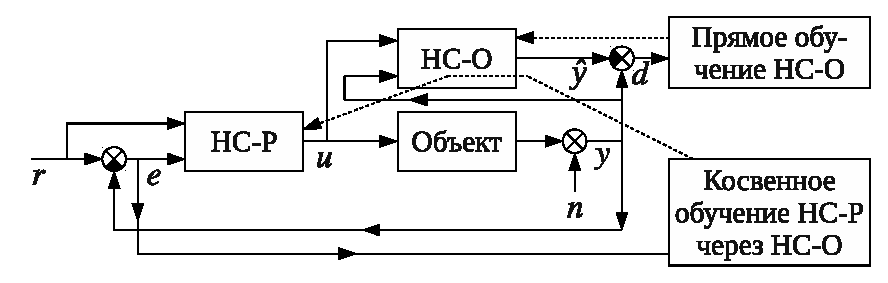
\includegraphics{permanent_adoption_rus}
\caption{������ ���������� �� ������ ���������� ���������.}
\label{fig:permanent_adoption_loop}
\end{figure}

�������� �������� ��������� ������� ���������� �������� ������� $r$ �
���������� ������ $n$ ������������ ������ �������.  ������������
��������� (��--�) ��������� �� ������ ���������� ����������� $u$ �
����� �������������� ������ ���������� $e=r-y$.  ����������� �������
�������� ��������� ���� �������������� (��--�), ������� �� ������������
����������� ���������� $u$ � ���������� ����������� ������ ������� $y$
������������� ����� ������� $\hat{y}$ � ��������� ������ �������.

������������ �������� ��� ��������� ��������� ��������� �����: ������
�������� ������������� �������������� �� ������ ������ �������������
$d=y-\hat{y}$ � ��������� �������� ������������� ���������� �����
��������� ��������������� ������ ���������� $e$ ����� ��--� � ��--�
(��. �.~\ref{nnc_optimal_training}).  ����������� ���������
��������������� ������ �������� �� ����� ����������� �������.

� ����� ���������� ��������� ������������ ��������� ���� �������
���������������.  ����������� ��������� ����� ���������� �
�������������� �������� �� \figref{fig:nonst_nn_schema}.  ��� �������
������������� �������� ������� ���������� �� ���� ��--� ��������
������� $u$ � $y$ ���������� ������� �������� ������� $D_u$ � $D_y$
�������������� (\figref{fig:nonst_nn_schema}�).  ������������
��������� �������� �� ���� �� ������ �������� ������ ����������, �� �
������� (\figref{fig:nonst_nn_schema}�).  ��� ������������ ��������
������������� ��� ���������� �������� ������ � ���������.

\begin{figure}[h]
\centering
\begin{tabular}{cc}
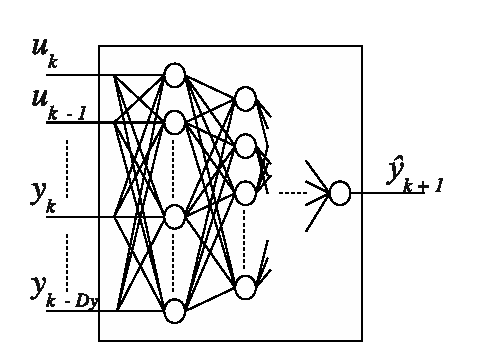
\includegraphics{nonst_nnp_schema} & 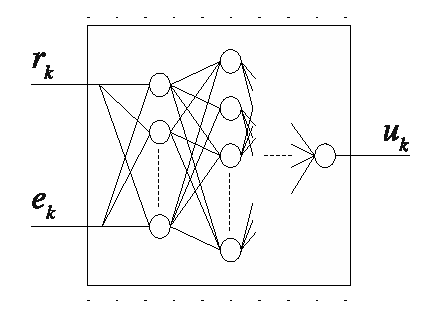
\includegraphics{nonst_nnc_schema} \\
�) & �)\\
\end{tabular}
\caption{����������� ��������� ����� ������ ������� (�) � ���������� (�).}
\label{fig:nonst_nn_schema}
\end{figure}

������� ����� �������� ��� ������ �������, ���������� ���������� �����
��������.  ��-������, � �������� ��������� ��������������� ������
���������� ����� ��������� �������������� �������� �������
������������� ��������������, �� �� �����������, ��������� ������
����������� ������ ���������� ����������� �� ��������� ����
����������, ��� ������� ������������ ���������� � ���� �����.
��-������, ������� �������� ��������� �������������� ��������
���������� �� �������� ����������, �� ����, �������� �������
������������� �������������� ���������� � �� ������ ���� �� �����.  �
������� �� �������� ��--� ��� ������� ����������
(��. ��.~\ref{nnpsynthesis} � \ref{nnp_series_req}), � ������ ������
�������� ���������� � ������� � �������� ������� � ��� �����������
�������.  � �������, ������������ ��������� ������� �������������
��������� ����� ����������� �� ���������� ���������� ������ ������
���������� ������� ���������� � ����������� (�������� ��������� ����)
� ��������� �������������� ������� ��������� ������.  ��� ���������
����������� �� �������������� ��������� ��������� �������
�������������.  �������� �������� ��������� ���� ��� �������
���������� ������ ����������� ��� ��������� �������� ��������, �� �
������ ������ ���� ������ ��������� ��������������� ������ ����������,
��������� ��������� ������������ ��������� ��--� ����� �������� �
������������� ��������� ��--�, � ��� ����� ������� ������ ����������
�� ������������.

\section{����� ��������� �� ����������� ��������}

������ �������� ���������� ������������� ���������� ��������
����������������� ������, ������� � ������������ �������� ��
������������ ��������� ��������� �����, ������ ��� ���� �������������
���� ����������� ��������� ������� ������� ���������� ---
��������~(\figref{fig:steady_state_loop}).  ����� ����������� ��������
�������������� ���� ����������� ������ � ������������ ��������
��������� ���� �������������� ��--� ��� ������� ����������.  ��
��������� �������� ������������� �������������� �� ���������� �
�������������� ����� ��������� ������������� ����������
��--�~(\figref{fig:modified_adoption_loop}) ���������� ����� �������
������������ ������������� ���������� � ������������ ������
(��. �.~\ref{nnc_optimal_training}).  ������� ��������, ��� �
������������ ����� ������������ ��������� ���� ��������� �����������
�����������, ��� � � ������ � ����������
����������~(\figref{fig:nonst_nn_schema}).

\begin{figure}[h]
\centering
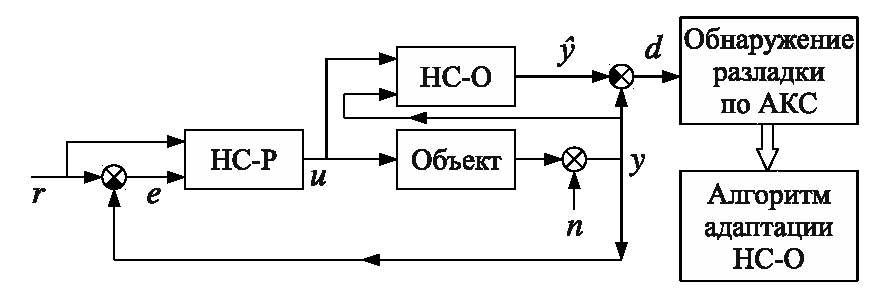
\includegraphics{steady_state_rus}
\caption{������ ���������� � ������������ ������.}
\label{fig:steady_state_loop}
\end{figure}

\begin{figure}[h]
\centering
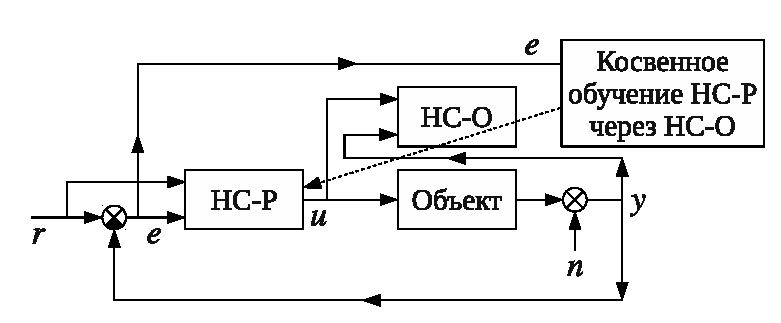
\includegraphics{modified_adoption_rus}
\caption{������ ���������� � ������ ��������� � ��������.}
\label{fig:modified_adoption_loop}
\end{figure}

��� ���� ����� ��� ����� �������� � �������������� ��������,
���������� ������� ���������� ������ ��������� ���������� �������
���������� � ��������� ������������ ��� ������������ ������.

������ ����������� �������� �������� � ������� ��������� ������������
���� (���), ������ ��� ���������� ����������� �������� ������� ������
������������ � �������� ���������� �������� ������� ������������.
���������� ������������ ������ ������� ���������� �������������� ���
������� ���������� ��������, ���������� � �.~\ref{nnpsynthesis}.  ���
�������� ��������� ���� � ���� ������ ���������� ����������� ���������
������ � ������, ����������� ��� ������������� ������������ ���������
������� � �������� ������������� ����������.  ��������� ��������������
�������������� �������� ��������� ��������� ����������, ����������
�������������� ������������ �������� ����� ������.  ���������� �������
���� ����� ����� ��������.

%\subsection{��������� ���}

% ������� ��� � ����������� ������������

��� ����������� ����������� ������� ��������� ����������� ��������
���������� ��������������� ��������� ���. ��� ��������, �������
����������� ���������� ������������� ��� �������� �������� �������
(�����) $H$ ({\em threshold}), � ��������� ���������������� ---
������� ����� ������������ $T_{ad}$ ({\em time of average alarm's
  delay}) � ������� ����� ����� ������� ��������� $T_{fa}$ ({\em time
  between false alarms}).  ������������� � ��������������� ������ ���
���������� �����, � ������� �������� ����� ������������ ������,
����������� � ���������� ��������� ���������� ������� ����������.

��� ��������� ��� ����� ������ �������� ��������������� ��������� �
�������� ��������� (�� ��������), ��������� �������� ����� ��
��������� ��� �������� (����������� ��������), � ����� ������� �����
$H>0$, �������������� �������� �������� $T_{ad}$ �
$T_{fa}$. ��������������� ������������ ��������, ��� � ��������
���������, �� �������� ������ ������������ ��������� ����������
������� ����������, ������� ������������ ��������� ������
������������� $d=y-\hat{y}$.  �� �������� �������� ������� �������
���������, ������������ ��� ������������� ������ $\sigma^2_0$, � ��
����������� �������� --- �� ���������� � �������� ����� ��� (��������,
$K=2$): $\sigma^2_1=K\sigma^2_0$.

��� ����������� �������� �� ��������� ���������� �������� � ����������
�������������� ��������� � ��������� ������������ ����� ���
����������� �� �������:
\begin{equation}
  z_i=-\frac{1}{2}\ln\frac{\sigma^2_1}{\sigma^2_0}-\frac{1}{2}
  \left(\frac{1}{\sigma^2_1}-\frac{1}{\sigma^2_0}\right)d_i^2
\end{equation}

���� ��������� ������������ ����� � ������������ ��� ��� ����������
������������ ����������� ��������� ����� ���:
\begin{equation}
  S_i=\left\{
  \begin{array}{ll}
    0, & i=0\\
    \max\left(0; S_{i-1}+z_i\right), & i>0\\
  \end{array}\right.
\end{equation}

��������� �������� ��������
\begin{equation}
  S_i>H
\end{equation}

\noindent �� ����, ���������� ������������ ������ $S_i$ ��������
������� $H$.  � ���� ������ �������� ��������� ������������,
������������ ����������� ��������� ������������� � ��� �������������
���������� ��������� ����������� ���������.  ��� ���� �����, ���
������ �������� ����� ����������� ���������� ���������� ����������
�������� � �������� ����������� ��������.  � ������ �������, �����
�������� ������ �������� � ����� ������� ������� ������������ � ����
����������� ��������.

��������� ��� �������������� ����� ������ $H$ ������ �� ����������
����������� ����� ���������� $T_{ad}$ � $T_{fa}$.  � ����� �����
�������� ����������� �������� ������������ ��������� � ������� �����
���������� ������� ���; ��� ���� �������� ��������� ��������������,
���� ������ � ��� ���������� � ��������� �� $3T_{ad}$.  �����
���������, ��� � ���� ������ ����������� ����� ������������
�����������.

��� ����������������� ��������� ��������� ����������� ��������
�������� ������� ������������� ��� ������ �� ���������� �������������
���������� ��������~\cite{filatov83,filfil-iwk1982}.  ������
������������ �������� ��������� �������������� ����������� �
������������ �� ���� �������� ������������� ���.  �������
�������������� ������� ���, ��� ������ ������������� � �����������
������� ���������� �������� ���������, �� ��������������� ���������.
������������ �������������� ����������� �������� ������� �����������
������������� $T_{ad}$ � $T_{fa}$ �� �������� ������ $H$ �
������������ �� ��� ��������� ��� (\figref{fig:nonst_atad},
\ref{fig:nonst_atfa}).

\begin{figure}[h]
\centering
\includegraphics[width=0.8\textwidth,%
  totalheight=0.35\textheight]{nonst_atad}
\caption{����������� �������� ������� ������������ $T_{ad}$ �� ������
  $H$ ��� ��������� ����������� �������� $K$.}
\label{fig:nonst_atad}
\end{figure}

\begin{figure}[h]
\centering
\includegraphics[width=0.8\textwidth,%
  totalheight=0.35\textheight]{nonst_atfa}
\caption{����������� �������� ������� ����� ������� ��������� $T_{fa}$
  �� ������ $H$ ��� ��������� ����������� �������� $K$.}
\label{fig:nonst_atfa}
\end{figure}

����� ��������� ������������� ������� � ���������� ��������� �����
����� ������������� ��������� ���������� ���, ����, � ���������,
���������� ��������� ������ �������������, ��������������� �����
������������ ���������.

%\subsection{������������ ��������� ������� � ��������� ��--�}

������������ ��������� ������� ��� ��������� ��--� � ������ �����������
�������� ����� ���� ���������, ��� ����������� � ������ �����
��������� ������� $N$ � � ������� �� ������������. ����������� ������
������������� ��������� ������� ���������� ����� � ������ ������
���������������.  ���� � ���, ��� ���������� ��--� ������ �������������
������ ��� ��� ��������� ������� � ������� ��������.  ������� � �����
������� ����� ������� �������������, ��� ������� ��������� �� �
����������� ������ � ���������� �������������� ����� ����� ����������.
���� �������, ��� ��� ������ ����� ��������� ������� ��� ����������
��--�, ���, � �����, ������������ ��� ����� ��������� �,
��������������, ������� � ������������ ����� ��������� ��--�.  ������
����������� �������� ������������ ��������� ������� ������
������������, ��������� ��� ������� ������������� ����������, � �����
� ��������� ������� ���� �������� � ������ ������������.

������������ ������������ � �������� �������������� ������� ��������
$\{u_k\}_N$ � $\{y_k\}_N$, ��������������� �� ��������� �� ������
������� ��������� �������������� ��������� ��� $t_0$ �� ������� $t_1$
��������� ������� � ������� �������� (��������� �� ���������� $M$)
���� $M$ ����������� ��������, ������� ����� �� ������� $t_0$, ��� ���
��� ���� ������ �������� � ������������� ������������ �������
��������� ���������� ��������.  ��������� ����� ��������� $t_1-t_0$
�������� ��������� ���������, � ���������� ����� �������� ���������
������� ��������� ����� $N=2M$.  ��� ����� ���������� �����������
������ ���������� ���������, ��������� ��� ��������� �������������
�������������� ��� ����� ����� ����������� ��������.

������ ������ ���� ������� ����� ��������� ������������� ���
������������� �������� ��--�, ���� ����� ��������� $t_1-t_0$ ����.
������������ �� ��� ��������� ������ ������� ��������� ����������
������������� $(u,y)$ � ����������� ����������� �������� $u_k,y_k$ ��
���������� ��������� ��������� ������� � �������� ����������.  ���
����������� ������������� ������ ������ ������� �� ������� $3\sigma$
������������ �������� �� �������.  ������ ��������� ���������
������������� ����� $(u,y)$ ���������� �� \figref{fig:u_ny_d2d_ru}.
�����, ��� ������������� ����� ����������� ���.

\begin{figure}[h]
\centering
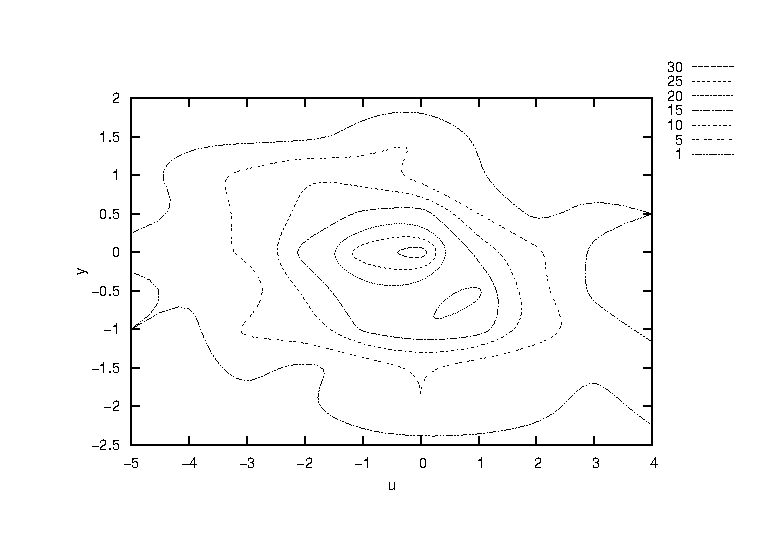
\includegraphics[width=0.8\textwidth,%
  totalheight=0.4\textheight]{u_ny_d2d_ru}
\caption{��������� ������������� $(u,y)$ � ���������� ������ ���������
  ��������.}
\label{fig:u_ny_d2d_ru}
\end{figure}

��������� �������� ��������� ����������� ������������ ���������
��������� ��� �������� ������������ ������������� ����������� �������,
��������������� ��������� ������� ����������.  ��� ��������� ���������
������������ ��� ��������� ��--� ��� ������� ����������.

\section{������������ � ����������� � �������������� ��������}

��� ���������� ������� --- ���������� ��������� (��) � � ���������� ��
����������� �������� (��) --- ���� ����������� � ������ ������������
������� ������������� � ������������� ����������.  ��� �������� ���
�������������� ������������� ��� �������� ������� � ���������
��������� ������ �������� ������������� ���������� � ����� �������.
��� ������ �������� ���� ����� ��� ��������: ��������������������
������ ����������, ������ ������������� �� ������������ �������, �
��������� ������������� ������ ����������, ��������������� �����������
������� �������� ������, ������� ������� ������� ���������� ��
�������������� ���������� �������.

%\subsection{������������ �������}

� ����� ������������� �� ������������ �������� ����������
������������� ��������� ������������ ������ ���������� � ��������, ��
��������� �������������.  ��� ������������� ������������� ���������� �
���������� ���������� ����������� ������������ ��������� ��������
���������� � �������� $2\times 10^5...5\times 10^5$ ������� �
���������� �� 0.05 �� 6. ��� ������ ����� �� �������
�������������������� ������ ����������
(\figref{fig:steady_plant_errors}).

\begin{figure}[h]
\centering
\includegraphics[width=0.7\textwidth,%
  totalheight=0.3\textheight]{perm_adopt_steady_plant_rus}
\caption{�������������������� ������ ���������� � ������������� �
  ������������ �������� ��� ���������� ��������� (��) � ��������� ��
  ����������� �������� (��).}
\label{fig:steady_plant_errors}
\end{figure}

������� ��������, ��� ��������� ������� �������������������� ������
������������� $d$ � ������ ���������� ��������� ����������� �
����������� ������ ����������.  ������������ ��������� � ������
����������������� ������� ��������� ����� ������ ���������
�������������������� ������ ���������� ����� �������� �������� 0.121.
��� ������������ ��������������� ������������� ������ ���������� ����
��������, ��� ��� ��������� �� ����������� �������� ������
������������ �� ������, ����� �������� � ����������� ������������
(\figref{fig:modif_apr_distrib_rus}).

\begin{figure}[h]
\centering
\includegraphics[width=0.7\textwidth,%
  totalheight=0.3\textheight]{modif_apr_distrib_rus}
\caption{������������� ������ ���������� ��� ��������� �� �����������
  �������� � ������������ ��������.}
\label{fig:modif_apr_distrib_rus}
\end{figure}

� ������ ���������� ��������� �������������� ������������� ������ ����
������������ � � ������� ��������� �������� ���������� �������
�������� ������ ������ ���������� �� ����.  ������� �������������
������ ���������� � ���� ��������� ���������� � ��� ���� �������
��������� �� \figref{fig:perm_adopt_distrib_rus}.  �����, ��� �
�������� ������� �������� �������� ���������� $[0, 4\times10^5]$
(\figref{fig:steady_plant_errors}) ������������� ������ � �����������,
������ � ������� ������� �������� ���������� (��������, $[4\times10^5,
  8\times10^5]$) ������������� ���������������.

\begin{figure}[h]
\centering
\includegraphics[width=0.7\textwidth,%
  height=0.3\textheight]{perm_adopt_distrib_rus}
\caption{������������� ������ ���������� ��� ���������� ��������� �
  ������������ ��������.}
\label{fig:perm_adopt_distrib_rus}
\end{figure}

�������������� ��������� ������������� ������ ���������� ������� �
\tablref{tabl:steady_state_distrib}.

\begin{table}
  \caption{��������� ������������� ������ ���������� � ������������ ��������.}
  \label{tabl:steady_state_distrib}
  \begin{tabular}{|l|c|c|c|c|}
    \hline
    & ������� & �������� & ������� & ���������\\
    \hline
    ���������� ���������&
    $-2.03$ & 5.43 & 0.33 & 0.30\\
    \hline
    ��������� �� ��������&
    $-1.46$ & 1.52 & $-0.01$ & 0.12\\
    \hline
  \end{tabular}
\end{table}

%\subsection{��������� ���������� ������� ����������}

� ������������� � �������������� �������� ���������� ��� ���������
������� �������� � ������ ������� 500.  ��
\figref{fig:nonst_cmp_pa_ma_rus} ������������ �������
�������������������� ������ ��� ���� ������ ����������: ����������
��������� ������������� ����������, ���������� ��������� ��--� � ��--� �
��������� ��--� ����� ����������� ��������, ����� ������ � ��������
��--� ��� �������.

\begin{figure}[h]
\centering
\includegraphics[width=0.7\textwidth,%
  height=0.3\textheight]{nonst_cmp_pa_ma_rus}
\caption{������������������� ������ ���������� � ������ ������
  ��������� ���������.}
\label{fig:nonst_cmp_pa_ma_rus}
\end{figure}

������� ��������� ���������� ������� � ������ ��������� �������������
���������� � ������ ������� � ���������� �� �������� ��������
������������� ������� � ���������.  �����, ��� ������������ ���������
� ���������� ���������� ��������� �� ��������� ������� ����������
������ � �� ���� ������ ���������� ������� ������ 0.55.  ������ �����
��������� ����� (�������� $10^4...10^5$) ������ ���������� ��������
����� ������� ����, ��� ����������� � ��� ������������ ��������.

����� � ���������� �� ����������� �������� ������� ����� ������ ���
��������� ������������� ����������.  � ������ ������������ �����
������� ��� �������� �������� 600 �������� �������.  �� ��� �����
�������������������� ������ ���������� ������ ������� �� 0.6.  �����
������� �������, ��� ��������� ������������� �������������� ���������
��������� (��� ������� �� �������� ������� �������� � ���������
�������������� ���������) � � ������ ������� 1100 �������� ���������
������������� ����������.  �� ��� ����� ������ ������� �� 0.7, ���
������ � ���������� ������������� ���������� ��� ���������.  �����
����� ������ ���������� ������ ���������� ���������, ������ ��������
�������� ���� ����������� ����, ��� � ������ ������� � ����������
����������.

�������������� ��������� ������ ���������� � �������� ���������
��������� � \tablref{tabl:nonst_state_distrib}.

\begin{table}
  \caption{��������� ������������� ������ ���������� � �������������� ��������.}
  \label{tabl:nonst_state_distrib}
  \begin{tabular}{|l|c|c|c|c|}
    \hline
    & ������� & �������� & ������� & ���������\\
    \hline
    ���������� ���������&
    $-12.31$ & 3.62 & $-5.23$ & 10.51\\
    \hline
    ��������� �� ��������&
    $-1.98$ & 2.00 & $-0.01$ & 0.46\\
    \hline
  \end{tabular}
\end{table}

\section{������}

\begin{enumerate}
\item ���������� ��� ������ ������������� ���������� ��������������
  ��������: � ���������� ���������� ���������� � ������, � ����� �
  ���������� �� ����������� ��������.  ��� ����������� �������� ��
  ��������� ������ ���������� ������������ �������� ������������ ����.
  ���������� ������ ������������� ����� ������ ��� ��������� ������
  ������� ����� ����������� ��������.
\item ��������� �������������� ������������ �� ���������� ������������
  �������� ������� ���������� � ����������� ����� �������.  ��������
  �������� ����� ������������� �������� ������������� ����������
  �������������� ��������.
\item �������� ������� �������������� � ������� ������������ ������
  ���������� � ���������� ���������� ������������� ���������� ��
  ��������� � ������� ��������� �� ����������� ��������.
\end{enumerate}


% Глава 6
\chapter{Нейросетевое управление мобильным роботом}
Как пример замены традиционного регулятора на нейросетевой для
управления реальным роботом.
%\input{part_mobile_robot.tex}

% Глава 7
\chapter{Программный пакет для моделирования и обучения методам нейросетевого управления}
%\centerline{Краткий план главы}
%\begin{enumerate}
%\item Цель работы: обучение и исследования
%\item Основные решаемые задачи
%\item Интеграция в учебный процесс и дидактические аспекты
%\item Описание лабораторных работ
%\item Описание программного комплекса
%  \begin{enumerate}
%  \item Структура комплекса и выбор инструментария
%  \item Основные интерактивные элементы
%  \item Вспомогательные интерактивные элементы
%  \item Сервисные и вычислительные программы
%  \item Объектная библиотека
%    \begin{itemize}
%    \item Абстракции данных и вспомогательный сервис.
%    \item Ввод-вывод, параметры.
%    \item Функциональные блоки от {\tt NaUnit} (+ .tf, .cof, .nn)
%    \item Нейросетевые элементы, методы обучения
%    \item Базовые структуры для построения сетей Петри
%    \item Объекты для моделирования дискретных динамических систем
%    \item Формализм для графического представления динамических моделей
%    \item Пример: дообучение нейросетевого регулятора в контуре
%    \item Пример: моделирование САУ и обнаружение разладки
%    \end{itemize}
%  \end{enumerate}
%\end{enumerate}

% -*-coding: utf-8;-*-
%%%%%%%%%%%%%%%%%%%%%%%%%%%%%%%%%%%%%%%%%%%%%%%%%%%%%%%%%%%%%%%%%%%%%%%%%%%%%%
% Программный комплекс для обучения методам нейросетевого управления в
% учебном процессе

% План:
% 1. Мотивация
%  1.1. Важность практических занятий в освоении НС
%  1.2. Почему новый пакет?
%  1.3. Состав лабораторных работ
%  1.4. Дидактические аспекты
% 2. Описание пакета
%  2.1. Перечень функций (смысловых, интерактивных)
%  2.2. Архитектура пакета
%  2.3. Выбор программной платформы
%  2.4. Описание объектной библиотеки и программ
% 3. Описание лабораторных работ
%  3.1. Синтез нейросетевого регулятора
%  3.2. Сравнение НС-Р, винервского оптимального и ПИД регулятора
%  3.3. Нейросетевое управление нестационарным объектом

%\section{Цель работы}

Применение нейронных сетей в системах управления является достаточно
новым направлением инженерной практики.  Исследования в этой области
идут широким фронтом, однако методологические аспекты пока
недостаточно проработаны.  В частности, это сказывается на том, что
отсутствуют общеизвестные программные пакеты, позволяющие изучать
нейросетевые методы автоматического управления не пользуясь
программированием.  Нет подходящих для этого и web-ресурсов.

В значительной мере это обусловлено тем, что теоретический базис по
нейронным сетям на настоящий момент не дает однозначных путей решения
многих прикладных задач.  До сих пор применение нейронных сетей --- во
многом эвристический процесс.  В таких условиях ВУЗовский учебный курс
по нейронным сетях обязательно должен включать практические занятия,
позволяющие студентам разобраться в недостаточно формализованном
предмете и получить необходимый опыт.

Представляется актуальным разработать интерактивный программный пакет
для настройки и моделирования традиционных и нейросетевых систем
управления с обратной связью.  Он был бы полезен как в рамках учебного
процесса в курсе нейронных сетей и курсе систем автоматического
управления на инженерных специальностях ВУЗов, так и в инженерной
практике при проектировании несложных систем управления.

На базе такого программного пакета можно разработать курс практических
работ, демонстрирующий возможности нейронных сетей в динамических
системах и сопутствующий лекционному материалу об использовании
нейронных сетей в системах управления.

%%%%%%%%%%%%%%%%%%%%%%%%%%%%%%%%%%%%
\section{Описание программного пакета}
% -*-coding: utf-8;-*-
%\section{Описание программного пакета}

\subsection{Основные решаемые задачи}

В соответствии со своим назначением программный пакет должен решать
задачи моделирования САУ, моделирования и обучения нейронных сетей.
Типовой сеанс работы с пакетом подразумевает интерактивное
взаимодействие пользователя с программами.  Поскольку пакет
разрабатывается для применения в учебном процессе, весьма желательно,
чтобы он был:
\begin{itemize}
\item простым в изучении и использовании;
\item адаптированным к специфике учебного процесса;
\item быстродействующим на не самых современных компьютерах;
\item открытым к модификации;
\item основанным на общедоступных и открытых технологиях.
\end{itemize}

При моделировании систем автоматического управления необходимо
предусмотреть возможность гибкой настройки контура и условий его
работы.  В частности, должны настраиваться:
\begin{itemize}
\item уставка (стохастическая, детерминированная);
\item помеха (стохастическая, детерминированная);
\item регулятор (линейный, нейросетевой);
\item объект управления (линейный, нелинейный, нестационарный).
\end{itemize}

%TODO: аргументировать, почему эти свойства важны.  м.б., в первой главе

В то же время, учитывая учебную направленность пакета, представляется
достаточным ограничиться одномерными системами управления когда объект
является одноканальным по входу и выходу.  Это существенно упрощает
интерактивную часть пакета и практику его использования.

Для моделирования и обучения нейронных сетей должны иметься следующие
возможности:
\begin{itemize}
\item создание нейронной сети с произвольной архитектурой в классе
  многослойных персептронов;
\item обучение нейронной сети на заданной выборке с контролем процесса
  по тестовой выборке;
\item предсказание поведения объекта управления с помощью нейронной
  сети в контуре в процессе моделирования;
\item обучение нейронной сети регулятора в контуре управления в
  процессе его моделирования.
\end{itemize}

Специфика применения нейронных сетей в системах автоматического
управления заключается в преимущественном использовании сетей класса
``многослойный персептрон'' с обучением методом обратного
распространения или более эффективными его вариантами.  По этой
причине нецелесообразно реализовывать поддержку сетей существенно иных
парадигм (Кохонена, Хопфилда и пр.).  Иногда применяемые в САУ
нейронные сети, основанные на радиально-базисных функциях (RBF),
доказанно являются эквивалентными многослойному персептрону, поэтому
их реализация тоже является избыточной и ради простоты программного
комплекса от неё целесообразно отказаться.

\subsection{Структура пакета и выбор инструментария}

Анализ требований к пакету обнаруживает, что некоторые из них трудно
совместить, пользуясь какой-то одной инструментальной технологией
разработки программ.  В частности, эффективное выполнение
вычислительных алгоритмов требует компиляции программ перед
выполнением.  Только с помощью компиляции можно обеспечить приемлемое
быстродействие на не всегда современных компьютерах, используемых в
учебном процессе.  В то же время, открытость к модификации
подразумевает возможность изменения программы прямо перед выполнением,
что важно для быстрой разработки, а также при углубленном изучении
пакета программ и проведении исследований с его помощью.

Кроме того, не все технологии разработки программного обеспечения
доступны на всех распространенных операционных системах: Microsoft
Windows, Linux, Mac OS X.  Некоторые из подходящих технологий
реализованы только в проприетарных программных продуктах,
использование которых требует покупки дорогостоящей лицензии.

В \tablref{tabl:sdk_tech} приводятся данные о сравнении нескольких
различных современных технологий разработки программного обеспечения
по перечисленным трем критериям.  Под технологиями в данном случае
понимается совокупность языка программирования, среды разработки и
выполнения и необходимые средства для реализации пользовательского
интерфейса и интерактивной графики.

\begin{table}[ht]
\centering
\caption{Сравнение технологий разработки программ.}
\label{tabl:sdk_tech}
\begin{tabular}{|l|c|c|c|}
\hline
\bf Технология & \bf Быстродействие & \bf Открытость к & \bf Общедоступность \\
             &                & \bf модификации  & \bf и открытость \\
\hline
             &                &  плохо       &              \\
\tt C++      &   отлично      & (требуется   & отлично      \\
             &                & компиляция)  &              \\
\hline
             &   средне       &  плохо       &              \\
\tt Java     & (интерпретация & (требуется   & отлично      \\
             & байт-кода)     & компиляция)  &              \\
\hline
             &   средне       &  плохо       & плохо        \\
\tt C$\#$    & (нужно много   & (требуется   & (в основном, \\
             & ресурсов)      & компиляция)  & для MS Windows) \\
\hline
            &   плохо        &              & средне       \\
\tt Python  & (интерпретация & отлично      & (нет унифициро- \\
            & байт-кода)     &              & ванной графики) \\
\hline
           &   плохо        &              &              \\
\tt Tcl/Tk & (интерпретация & отлично      & отлично      \\
           & байт-кода)     &              &              \\
\hline
           &   средне       &              & плохо        \\
\tt Matlab & (интерпретация & отлично      & (платный и   \\
           & байт-кода)     &              & очень дорогой) \\
\hline
\end{tabular}
\end{table}

Отсутствие идеальной технологии для разработки пакета моделирования и
нейросетевого управления вынуждает искать компромиссное решение.
Можно функционально разделить пакет на интерактивную и вычислительную
части и реализовать каждую с помощью оптимальной технологии.
Вычислительная часть требует эффективной реализации с точки зрения
быстродействия, поэтому целесообразно реализовать её на языке {\tt
  C++}.  Компиляторы этого языка программирования доступны для всех
значимых платформ, а сам язык, пожалуй, является в настоящее время
наиболее популярным среди универсальных процедурных языков
программирования.

Интерактивную графику и управление вычислительными алгоритмами важно
сделать максимально гибкими и открытыми для модификации.  Хорошим
выбором будет использование интерпретируемого языка с встроенными
возможностями для реализации пользовательского интерфейса, прикладной
графики и средствами интеграции программного обеспечения.  Одним из
подходящих инструментов является {\tt Tcl/Tk}, доступный бесплатно и в
исходных текстах для всех распространенных операционных систем.

Функциональная декомпозиция разрабатываемого пакета по используемым
технологиям разработки программ находит отражение в структуре
взаимодействия отдельных частей программного комплекса, которая
приводится на \figref{fig:prog_interaction_struct}.  Реализация
вычислительных функций в отдельных узкоспециализированных программах,
написанных на языке {\tt C++}, позволит пользователю гибко управлять
их взаимодействием и во многих нестандартных случаях снизит
необходимость в модификации текстов на {\tt C++}.

\begin{figure}
\centerline{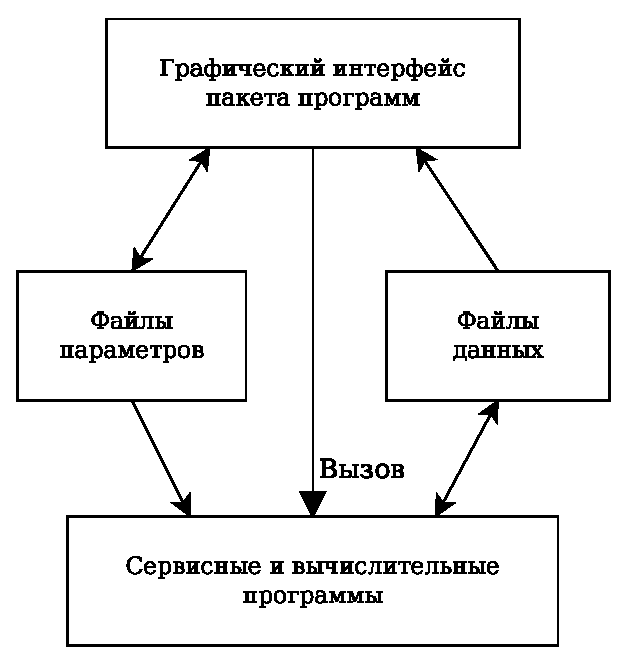
\includegraphics{princ_struct.eps}}
\caption{Схема взаимодействия частей программного пакета}
\label{fig:prog_interaction_struct}
\end{figure}

\subsection{Основные интерактивные элементы}

Интерактивная часть пакета разрабатывается с использованием парадигмы
событийно-управляемого программирования.  Действия пользователя
порождают события, которые, в свою очередь, приводят к вызову
процедур, ассоциированных с ними.  Структура событийно-управляемой
программы имеет следующие особенности:
\begin{itemize}
\item Основной структурирующей единицей программы является окно.
\item Перед появлением окна на экране выполняется программный код ---
  процедура инициализации окна, --- формирующий внешний вид и основные
  интерактивные возможности взаимодействия с этим окном.
\item Внешний вид окна и его поведение может зависеть от параметров
  процедуры инициализации.
\item Процедуры-обработчики событий устанавливаются при создании окна
  или в процессе его жизни.
\item Внешний вид окна и его поведение в течение жизни может зависеть
  от действий, выполняемых в тех или иных обработчиках сигналов.
\end{itemize}

В соответствии с поставленными задачами целесообразно распределить
функции программы между окнами пользовательского интерфейса со
следующим назначением:
\begin{enumerate}
\item моделирование системы автоматического управления включая случай
  нестационарного поведения объекта;
\item создание/просмотр/редактирование цепочки линейных и нелинейных
  звеньев;
\item создание/просмотр/редактирование нейронной сети;
\item обучение нейронной сети модели объекта управления с
  использованием указанных выборок вне контура;
\item обучение нейронной сети регулятора с использованием указанных
  выборок вне контура;
\item обучение нейронной сети регулятора в контуре управления в
  процессе его моделирования;
\item просмотр заданных выборок (дискретных временных рядов) в виде
  графиков по времени;
\item просмотр заданной выборки в виде гистограммы для оценки
  одномерного распределения;
\item просмотр двух заданных синхронных выборок в виде множества точек
  на двумерной плоскости для оценки двумерного распределения.
\end{enumerate}

\subsection{Сервисные и вычислительные программы}
% TODO: перечислить наименование и назначение ряда программ

В соответствии с разработанной схемой взаимодействия компонентов
пакета моделирования (\figref{fig:prog_interaction_struct}) основные
блоки, выполняющие численные расчеты и обработку данных, не связанную
непосредственно с визуализацией графики, реализуются на языке
программирования {\tt C++} набором неинтерактивных программ.  Эти
программы взаимодействуют друг с другом и с пользовательским
интерфейсом не непосредственно, а через файлы параметров и данных.

Управление работой программ поизводится путем задания всех необходимых
параметров перед их запуском.  В различных программах в зависимости от
сложности их параметризации реализованы следующие способы передачи
параметров:
\begin{itemize}
\item в качестве аргументов командной строки;
\item через переменные рабочего окружения;
\item через файл с параметрами.
\end{itemize}

Конфигурационные файлы с параметрами различных программ имеют общий
синтаксис, описанный в \tablref{tabl:par_syntax}.

\begin{table}[ht]
\centering
\caption{Описание формата файла параметров.}
\label{tabl:par_syntax}
\begin{tabular}{|c|l|p{10cm}|}
\hline
Правило & Синтаксис & Семантика \\
\hline
1 & \tt \#                 & Однострочный комментарий \\
2 & \tt \em Имя = Значение & Параметр с заданным именем и значением до конца строки \\
\hline
\end{tabular}
\end{table}

Перечень вычислительных и сервисных программ с классификацией по
областям назначения приведен в \tablref{tabl:prog_list}.

\begin{table}%[ht]
\centering
\caption{Список вычислительных и сервисных неинтерактивных программ пакета.}
\label{tabl:prog_list}
\begin{tabular}{|c|l|p{13cm}|}
\hline
N^0 & Название & Назначение \\
\hline
\hline
\multicolumn{3}{|c|}{Основные программы моделирования и специализированного обучения нейросетей} \\
\hline
1 & \tt dcsloop & Моделирование контура управления. \\
2 & \tt dplantid & Обучение нейросетевой модели объекта управления вне контура  \\
3 & \tt dnnplant & Проверка функционирования нейросетевой модели объекта \\
4 & \tt dcontrp & Предварительное обучение нейросетевого регулятора подобно заменяемому вне контура управления \\
5 & \tt dcontrf & Дообучение нейросетевого регулятора в контуре управления с помощью нейросетевой модели объекта \\
\hline
\multicolumn{3}{|c|}{Неспециализированная работа с нейронными сетями} \\
\hline
6 & \tt MakeNN & Подготовка файла нейронной сети заданной архитектуры \\
7 & \tt ResetNN & Инициализация весовых коэффициентов нейронной сети случайными значениями \\
8 & \tt TrainNN & Обучение нейронной сети общего вида на заданных примерах \\
9 & \tt EvalNN & Проверка работы настроенной нейронной сети общего вида \\
\hline
\multicolumn{3}{|c|}{Генерация временных рядов} \\
\hline
10 & \tt dmeander & Генерация временного ряда вида ``меандр'' \\
11 & \tt drand & Генерация случайного временного ряда с заданными параметрами \\
12 & \tt drandmea & Генерация случайного временного ряда вида ``меандр'' с заданными параметрами \\
13 & \tt dsin & Генерация моногармонического временного ряда с заданными параметрами \\
\hline
\multicolumn{3}{|c|}{Операции с временными рядами} \\
\hline
14 & \tt dmult & Умножение значений временного ряда на указанное число \\
15 & \tt dsub & Вычитание значений временных рядов \\
16 & \tt dsum & Сложение значений временных рядов \\
\hline
\multicolumn{3}{|c|}{Обработка и изучение временных рядов} \\
\hline
% & \tt d2ts & Нумерация значений временного ряда \\
17 & \tt dconst & Проверка гипотезы о постоянном среднем значении временного ряда \\
18 & \tt dcorr & Расчет функции корреляции указанной длины для заданных временных рядов \\
% & \tt djacob & Расчет дискретной оценки якобиана по временным рядам управляющего сигнала и состояния одномерного объекта \\
19 & \tt dmean & Расчет среднего значения временного ряда \\
20 & \tt dmse & Расчет среднеквадратичной ошибки временного ряда \\
% & \tt dsmooth & Сглаживание временного ряда на скользящей базе  \\
% & \tt dstat & Расчет статистических параметров временного ряда нарастающим итогом \\
% & \tt dstatsb & Расчет статистических параметров временного ряда в скользящей базе \\
21 & \tt dstddev & Расчет среднеквадратичного отклонения временного ряда \\
22 & \tt dtf & Применение заданной линейной передаточной или комбинированной функции к указанному временному ряду  \\
23 & \tt Distr1D & Построение одномерного распределения временного ряда \\
24 & \tt Distr2D & Построение двумерного распределения временного ряда \\
% & \tt FileCvt & Преобразование формата файла временного ряда \\
25 & \tt StatAn & Расчет статистических параметров временного ряда \\
\hline
\multicolumn{3}{|c|}{Алгоритм кумулятивных сумм} \\
\hline
26 & \tt acstest & Проверка параметров АКС вне контура управления \\
\hline
\end{tabular}
\end{table}


\subsection{Объектная библиотека}

Объектно-ориентированная библиотека {\tt NeuArch} разработана на языке
программирования {\tt C++} и предназначена для реализации следующих
основных задач:
\begin{enumerate}
\item Работа с цепочками линейных и нелинейных звеньев: создание,
  выполнение, хранение в файлах.
\item Работа с нейросетями архитектуры ``многослойный персептрон'':
  создание, обучение, выполнение, хранение в файлах.
\item Моделирование динамических систем в дискретном времени.
\end{enumerate}

Кроме того, библиотека реализует ряд необходимых вспомогательных
функций: ввод/вывод временных рядов, чтение и запись файлов
параметров, абстрактные структуры данных и прочий сервис.

Библиотека является переносимой (функционирует на ОС MS Windows и
Linux) и универсальной, то есть, не содержит буквальной реализации
высокоуровневых функций, возложенных на программный пакет.

\subsubsection{Моделирование линейных звеньев}

Для моделирования на компьютере системы управления в целом необходимо
иметь компьютерные модели составных элементов.  Для описания линейного
элемента удобно воспользоваться z-преобразованием передаточной
функции.  Это представление является общепринятым в классе линейных
систем в дискретном времени.

В программном пакете передаточная функция $P^*(z)$ линейного элемента
описывается произвольной комбинацией следующих базовых конструкций:

\begin{equation}\label{eq:polyfrac}
P^*(z)=\frac{a_nz^n+a_{n-1}z^{n-1}+...+a_0}{b_mz^m+b_{m-1}z^{m-1}+...+b_0}
\end{equation}
\begin{equation}\label{eq:sum}
P^*(z)=\sum\limits_{i=1}^NP^*_i(z)
\end{equation}
\begin{equation}\label{eq:product}
P^*(z)=\prod\limits_{j=1}^MP^*_j(z)
\end{equation}

Несмотря на то, что действующую линейную передаточную функцию всегда
можно привести к полиномиальному виду \ref{eq:polyfrac}, удобно иметь
возможность произвольного описания.  Можно подобрать такую структуру
представления линейного элемента, чтобы коэффициенты имели легко
интерпретируемый смысл.  Например, ПИД регулятор удобно задавать в
виде суммы произведений полиномиальных дробей:

\begin{equation}\label{eq:pid}
C_{PID}^*(z)=K_P+K_I\frac{z}{z-1}+K_D\frac{z^2-2z+1}{z^2-z}
\end{equation}

В этом случае коэффициенты $a_0$ вырожденных полиномиальных дробей
$\frac{a_0}{1}$ приобретают общеизвестный смысл $K_P$, $K_I$ и $K_D$.

Пример представления конкретного ПИД регулятора

\begin{equation}\label{eq:pid_example}
C_{PID}^*(z)=-0.3+1.47\frac{z}{z-1}+0.02\frac{z^2-2z+1}{z^2-z}
\end{equation}

\noindent в формате, воспринимаемым пакетом моделирования, приводится ниже:

\begin{verbatim}
;NeuCon transfer 1.0
; Speed form of a discrete PID controller
[TransferFunction]
sum 3		 ; Kp + Ki*(z/z-1) + Kd*(z2-2z+1/z(z-1))
polyfrac 0	 ; <=== Proportional term
 -0.3 /  1	 ; Kp
product 2	 ; <=== Integral term
polyfrac 0
 1.47 /  1	 ; Ki
polyfrac 0
 1 0 /  1 -1
product 2	 ; <=== Differencial term
polyfrac 0
 0.02 /  1	 ; Kd
polyfrac 0
 1 -2 1 / 1 -1 0
\end{verbatim}

Синтаксис файла кратко описан в \tablref{tabl:tf_syntax}.  Комбинация
полиномиальных дробей с помощью операций суммирования и произведения
осуществляется с помощью префиксной формы записи.  Текстовый формат
файла позволяет легко редактировать его в любом редакторе.

\begin{table}[ht]
\centering
\caption{Описание формата файла задания линейной передаточной функции.}
\label{tabl:tf_syntax}
\begin{tabular}{|c|l|p{9.5cm}|}
\hline
Правило & Синтаксис & Семантика \\
\hline
1 & \tt ;NeuCon transfer 1.0 & Служебный комментарий в первой строке файла \\
2 & \tt ;                    & Признак комментария до конца строки \\
3 & \tt [TransferFunction]   & Признак начала описания передаточной функции \\
4 & \tt polyfrac $A$           & Признак начала описания на следующей строке \\
  & $a_n\:a_{n-1}\:...\:a_0$ {\tt /} $b_m\:b_{m-1}\:...\:b_0$ & коэффициентов (см. \ref{eq:polyfrac}).  $A$ произвольное число. \\
5 & \tt sum $N$              & Признак начала описания суммы из $N$ идущих следом описаний по правилам 4--6 (см. \ref{eq:sum}) \\
6 & \tt product $M$          & Признак начала описания произведения из $M$ идущих следом описаний по правилам 4--6 (см. уравнение \ref{eq:product}) \\
\hline
\end{tabular}
\end{table}

Линейные передаточные функции используются в пакете для моделирования
регуляторов и объектов управления, а также для формирования из
случайной последовательности --- белого шума --- временных рядов
уставки и помехи с заданными корреляционными свойствами.

\subsubsection{Моделирование нелинейных звеньев}

Нелинейные звенья в силу их потенциально бесконечного разнообразия
реализуются в небольших динамически подключаемых предварительно
скомпилированных внешних библиотеках.  Способ создания, подключения и
параметризации таких библиотек очень прост и унифицирован для того,
чтобы можно было расширять список реализованных в пакете нелинейных
звеньев (см. \figref{fig:nonlinear_functions}) произвольными новыми,
которые требуются в конкретном исследовании или учебной работе.
Поскольку вид реализованной функции пакету неизвестен, правильнее
говорить о реализации во внешних библиотеках пользовательских функций.

\begin{figure}[h]
\centering
\begin{tabular}{cc}
\includegraphics{func_nosense.eps} &
\includegraphics{func_saturat.eps} \\
а) Зона нечувствительности ({\tt nosense})& б) Насыщение ({\tt saturat}) \\
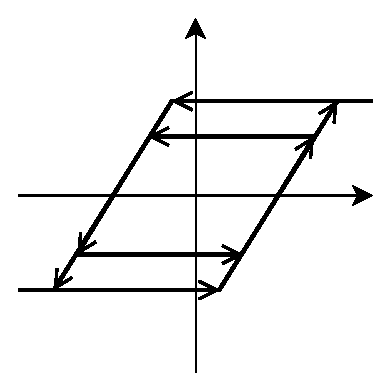
\includegraphics{func_luft.eps} &
\includegraphics{func_sine.eps} \\
в) Люфт ({\tt luft}) & г) Синус ({\tt sine}) \\
\end{tabular}
\caption{Реализованные в пакете нелинейные звенья.}
\label{fig:nonlinear_functions}
\end{figure}

Количество нелинейных звеньев в пакете намеренно сделано небольшим.
Расширение списка нелинейных звеньев может быть предложено студентам в
качестве одного из направлений учебно-научной работы.

Нелинейные звенья могут комбинироваться с линейными в любом порядке.
Пример файла, задающего функцию объекта в виде инерционного звена
первого порядка $I^*(z)=\frac{1.6z}{z-0.7}$ с зоной
нечувствительности, приводится ниже:

\begin{verbatim}
;NeuCon combined function 1.0
[CombinedFunction main]
TransferFunction inert
CustomFunction deadzone

[CustomFunction deadzone]
; Extension:   .so/.dll depending the OS
file    nosense
;HalfWidth Gain
options 0.5 2
;Initial vector (may be empty)
initial

[TransferFunction inert]
polyfrac 0
 1.6 0 /  1 -0.7
\end{verbatim}

Краткое описание формата файла комбинированной функции приводится в
\tablref{tabl:cof_syntax}.

\begin{table}[ht]
\centering
\caption{Описание формата файла задания комбинированной функции.}
\label{tabl:cof_syntax}
\begin{tabular}{|c|l|p{8cm}|}
\hline
Правило & Синтаксис & Семантика \\
\hline
1 & \tt ;NeuCon combined function 1.0 & Служебный комментарий в первой строке файла \\
2 & \tt ;                    & Признак комментария до конца строки \\
3 & \tt [CombinedFunction \em Имя \tt] & Признак начала описания комбинированной функции, действующей в порядке перечисления \\
4 & \tt TransferFunction \em Имя & Ссылка на линейную функцию {\em Имя} \\
5 & \tt CustomFunction \em Имя & Ссылка на пользовательскую функцию {\em Имя} \\
6 & \tt [TransferFunction \em Имя \tt] & Признак начала описания передаточной функции (см. \tablref{tabl:tf_syntax})\\
7 & \tt [CustomFunction \em Имя \tt] & Признак начала описания пользовательской функции \\
8 & \tt file \em ИмяФайла & Имя файла без расширения ({\tt .so} или {\tt.dll}) с библиотекой, реализующей функцию \\
9 & \tt options \em Параметры & Перечень числовых параметров функции (через пробел) \\
10 & \tt initial \em Инициализация & Перечень чисел для инициализации начального состояния функции (через пробел) \\
\hline
\end{tabular}
\end{table}


\subsubsection{Нестационарные элементы моделирования}

Нестационарное поведение объектов моделирования реализуется в
программном пакете двумя способами:
\begin{enumerate}
\item с помощью специально запрограммированного звена, обладающего
  нестационарными свойствами;
\item заданием списка функций и времени переключения с одной функции
  на другую.
\end{enumerate}

Первый способ более общий.  Он позволяет реализовать произвольное
поведение объекта, например, плавное изменение параметров.  Однако он
требует запрограммировать необходимые действия и скомпилировать
полученный программный модуль в виде внешней пользовательской
библиотеки, что не всегда удобно и ведет к дополнительному расходу
времени.

Второй способ позволяет описать в текстовом файле комбинированной
функции правило, по которому будет изменяться функция объекта.
Правило задается перечнем функций и периодами времени, в которые эти
функции реализуют поведение объекта.  В целом, для функций $g_i()$ и
моментов времени $t_i$ правило вычисления действующей функции объекта
описывается формулой:

$$
y=\left\{
\begin{array}{ll}
  g_1(t,x), & 0\le t < t_1\\
  g_2(t,x), & t_1\le t < t_2\\
  ... & \\
  g_l(t,x) & t \ge t_l
\end{array}\right.
$$

\noindent где все $t_i$ кратны шагу дискретизации по времени в сеансе
моделирования.

Например, если надо запрограммировать изменение коэффициента усиления
c 1.5 на 3.4 в момент времени $t=500$, это можно описать в файле
следующей комбинированной функцией:

\begin{verbatim}
;NeuCon combined function 1.0
[CombinedFunction main]
TransferFunction k1 0 500
TransferFunction k2 500 -1

[TransferFunction k1]
polyfrac 0
 1.5 /  1

[TransferFunction k2]
polyfrac 0
 3.4 /  1
\end{verbatim}

\subsubsection{Нейронные сети и методы их обучения}
\subsubsection{Моделирование динамических систем}



\subsubsection{Объекты для моделирования дискретных динамических систем}
\subsubsection{Формализм для графического представления динамических моделей}
\subsubsection{Пример: дообучение нейросетевого регулятора в контуре}
\subsubsection{Пример: моделирование САУ и обнаружение разладки}


%%%%%%%%%%%%%%%%%%%%%%%%%%%%%%%%%%%%
\section{Применение пакета в курсе лабораторных работ}
% -*-coding: cp1251;-*-
%\section{���������� ������ � ����� ������������ �����}

�� ���� �������������� ������������ ������ ������������� �
��������������� ������������ � ������������ ������ ���������� ���
���������� ���� ������������ �����.  ���� ���� �������������, � �����
�������, ����������� ���������� ��������� ����� ��� ������� ���������
����� ��������������� ����������, � ������ �������, �����������
������������ ������ ��� ������������� ��� � �������� ��������� �����.

%\subsection{���������� � ������� �������}

��������������� ���� ������������ ����� ������������ ��� ����������
������������� �����, ������������ ���������� ������������� ���������
����� � �����.  � ������ ��������� ����������� �� ������� ��
������������ ������� ���������� �������� ��� ������������ �������
������������� 3--4 ���� ������.  �������������� �����������
������������ ������� �������� � ������� �� ��������� �����:

\begin{itemize}
\item ������ ������������� ������������ ����������.
\item ������������� ������ �������������, ������������ � ��� �����������.
\item ������������ ���������� �������������� ��������.
\end{itemize}

������ ������������ ������ ����������� �������� ������ ���������� �
������������ ������� ���������� �� ������������.  ��� ����� ����������
�������� ������������� � ������� ������ ��� ���������� ��������
������������� ���������� � ������ �������.  ����� ����� ���������
��������� ��������� ���� ���������� � ������ �������.  ��������������
����������� ��������� ���������� � ��� �� ����� ��������� � � �������
������ ������� � �������� ������ �������������� ��� ����������� ������
����������.

� ������ ������ ������ ��������� �������� ����������� ������������
��������� � ����������� ����������� � ��� ����������� � ���������
��������, ��� ����������� (������������ ��� ���������), ��� �
������������ �� ���.  � ���������, ������� �������� ������������� �
������� ������ �������� ������� � �������������� ������,
���������������� ����������� ����������� �������� ���������� ��
�������, ����������, ��������� ������������ ��������� � ��������
������� ���������� ������� ����������.

������ ������������ ������ ��������� ������ ������������� ����������
�������������� ��������.  ��� �������� ��������� ������� �����������
�������� � ������� ������������ ������ � ��������� ������������ ����
(���), ���� ������ � ���������� � �� ������� ������ �������
����������, � ����� ���������� ������������� ���������� � �������.

�������� ������������ ����� ���������� ������������.  � ���������,
��������������� ��� ��������������� (������ ��������� ���, �����������
���), ��� � ����������������� ������ (����� ����������� �����������
���������, ��������� ��������� �����������).  ������������� �
��������� ������������, � ��� �����, � ����������� �����������,
��������� �������� ����� � ������������ ������� ���������������
����������.  ������������� ��� ��� ����������� �������� �������������
����������� ����������� ������������� ������������ � ������������
����������.

%\subsection{������������� �������}

�������� ���������� ������������ ������ ������� �� �������� ���������
����� ������������:

\begin{itemize}

\item �������� ������������� ����� ��������� �����;

\item �������� ������������ ���������;

\item ���������� ������.

\end{itemize}

��������, �������� � ������������ ������, �������������, ��� ������
������������� ������ ���������� ����� ����� ������� �������� ��������
�� �������������� ����������, ������ ������� ������������ �����������
� �������� ������ ��������������� ���������� (��� ����������������� �
�������������� ��������).

� ���������� ���������� ������������ ����� ������� ������ �������:
\begin{itemize}

\item ����������� ��������� ����� ������� ���������������.

\item ������� ���������� ���������� ������ ������������ �������
  ��������� ��� ($\{{e_k,r_k}\}$, $\{e_k,e_{k-1},...\}$,
  $\{u_k,u_{k-1},...y_k,y_{k-1},...\}$).

\item ������� ���������� �������� �������� ����������, �������������
  ��� ��������� ����������, �� ���������������� ��� � ��������,
  ������������ � �������� (������, �������� �������������� �������� �
  ������� ����������, ����������������).

\item ����� ��������� ��������������� ������ � ��� ���������� ���
  ������� ��������� ������������ ������� ���������� (���������
  ��������� � ���������� � ������� ������������� ����������, ���������
  ������������ ������ ������� ����������).

\item ���� ������������ ������ ������� ��� ������� �������������
  ���������� � ��� ����������� ��������.

\item ������� ��������� � ����������� ������ �� �������� ���������
  ��������� ���� (������� ����������� � ������� �������� ���������).

\item �������� �������� ������������ ����������� � �� ������� ��
  �������� ����������� (��������� ��������������, ����������� ��
  ������ ��������, ������������, ���������������� � ����������
  �������� � ��.).

\item ������ ������������� ���������� �������������� �������� � ��
  ����������� (��������������, ��������������, ������������).

\end{itemize}


%%%%%%%%%%%%%%%%%%%%%%%%%%%%%%%%%%%%
\section{Описание лабораторных работ}
% -*-coding: utf-8;-*-
%%%%%%%%%%%%%%%%%%%%%%%%%%%%%%%%%%%%%%%%%%%%%%%%%%%%%%%%%%%%%%%%%%%%%%%%%%%%%%
% Программный комплекс для обучения методам нейросетевого управления в
% учебном процессе

\section{Цель работы}


Разработка интерактивного программного комплекса для настройки и
моделирования традиционных и нейросетевых систем управления с обратной
связью.

Преподавание нейросетевых методов на инженерных специальностях должно учитывать специфику 


\subsection{Мотивация}

Искусственные нейронные сети представляют собой относительно новый
мощный и многогранный инструмент для решения разнообразных инженерных
и научно-исследовательских задач.  Способ применения нейронных сетей
достаточно специфичен, так как он основан не на аналитическом
формализме, а на обучении --- неявном извлечении взаимосвязей из
представленных данных.  Эта особенность отличает нейросетевые методы
от традиционных в том числе и в задачах автоматического управления.

Аналитические методы давно и прочно укоренились в учебных курсах на
инженерных специальностях.  Для освоения аппарата этих методов
студентам предлагается большое количество разнообразных упражнений,
суть которых сводится к аналитическому решению задачи, то есть, к
выводу формальным способом решения в общем виде.  Только в том случае,
если математический аппарат не позволяет получить чточное решение в
аналитической форме, используются приближенные способы решения, в том
числе, с помощью численных методов.  Однако в любом случае вид
решения, а значит и его свойства, определяются человеком.

Нейросетевые методы подразумевают участие человека только в
обеспечении процесса обучения, а собственно решение формируется
нейросетью само.  Его вид и свойства изначально неизвестны.  Более
того, после успешного завершения обучения нейронной сетью, отличной от
тривиальной, человеку практически невозможно понять, какие решения
приняла сеть и и как это повлияло на достижение поставленной цели.
Иногда даже говорят о самостоятельной задаче извлечения знаний из
обучечнной нейронной сети.

Написать про неполноту формального описания ИНС.

Изложенные особенности свидетельствуют об особой важности практических
работ в учебном курсе по нейросетевым методам.  Только они дают
возможность студентам увидеть, как происходит процесс обучения и как
функционирует обученная нейронная сеть в рамках решения конкретной
прикладной задачи.  Это невозможно до конца формализовать на лекциях и
изложить в учебных пособиях.  Фактически, совокупность архитектуры НС,
метода обучения с его параметрами, а также обучающих данных дает
уникальное решение, выражающееся в наборе весовых коэффициентов НС.

Обычно для практических работ по курсу искусственных нейронных сетей
используется тот или иной универсальный (Statistica, MatLab, Octave)
или специализированный нейросетевой (Stuttgart Neural Network
Simulator, Neural Lab, Trajan) программный пакет.  Для большинства
типовых задач, решаемых с помощью НС (распознавание образов,
ассоциативная память, кластеризация и т.п.), возможностей
перечисленных пакетов вполне достаточно.  К ним относятся:

\begin{itemize}
\item Задание архитектуры нейросети и метода её обучения
\item Задание обучающего множества
\item Задание параметров обучения
\item Обучение нейронной сети
\item Анализ качества работы обученной нейронной сети
\end{itemize}

Однако применение НС в задачах управления требует дополнительно
наличия многих функций, отсутствующих в пакетах нейросетевого
моделирования:

\begin{itemize}
\item Задание вида и параметров регулятора и объекта управления
\item Задание входных сигналов - уставки и помехи
\item Съем данных из различных точек контура управления для
  визуализации и обучения НС
\item Моделирование САУ
\item Сравнение и анализ качества работы САУ с различными
  компонентами, в том числе, с нейросетевыми
\end{itemize}

В универсальных же пакетах (класса MatLab) реализация перечисленных
функций требует достаточно серьезного программирования как
вычислительных, так и интерактивных и графических функций.  В то же
время, получающаяся программа обладала бы ограниченным
быстродействием, так как должна быть написана на интерпретируемом
языке программирования.  Вопросы быстродействия в данном классе задач
достаточно важны, так как моделирование и обучение нейронных сетей
производится на длинных временных рядах (порядка $10^4 ... 10^6$
отсчетов).

Представляется актуальным разработать интерактивный пакет программ,
позволяющий решать задачи нейросетевого управления и сопоставлять
нейросетевые подходы с традиционными.  На базе такого пакета можно
создать курс практических занятий для студентов инженерных
специальностей, изучающих применение нейронных сетей в системах
автоматического управления.  Подобный программный комплекс был бы
полезен и для исследовательских проектов, позволяя быстро провести
моделирование проектируемой САУ и оценить возможности использования в
ней нейросетевого управления.


\section{Постановка задачи}
Фактически, Т.З. на три лабораторных работы:
\begin{itemize}
\item Синтез нейросетевого регулятора
\item Сравнительный анализ нейросетевого, винеровского и ПИД регуляторов
\item Управление нестационарным объектом
\end{itemize}

Совершенствование лабораторной базы.  Предлагается создать лабораторные работы.

Программный комплекс.
Задачи, возложенные на этот комплекс.

\subsection{Структура комплекса}
\subsection{Принципы взаимодействия}

\subsection{Дидактические цели}
Что должен знать и уметь студент по результатам выполнения лабораторных работ.

\subsection{План методички}
\begin{itemize}
\item Введение: цель работы
\item Теоретическая часть - взять из 2, 3, 4 глав
\item Задание на выполнение работы
\item Инструкция по проведению работы (описание программного комплекса)
\item Представление результатов
\item Контрольные вопросы
\end{itemize}

\section{Методическая база}
\subsection{Примеры отчетов - в приложении}


%%%%%%%%%%%%%%%%%%%%%%%%%%%%%%%%%%%%
\section{Выводы}
% -*-coding: cp1251;-*-
%%%%%%%%%%%%%%%%%%%%%%%%%%%%%%%%%%%%%%%%%%%%%%%%%%%%%%%%%%%%%%%%%%%%%%%%%%%%%%

\begin{enumerate}
\item ���������� ������������� ����������� �������� �������������
  ������������� ��� � ���������� ������� � ������������ �������������
  ��������, ���������� � �������������� �������� � �����������, �
  ����� ��������� �����, ������� ��������� �� ��������..
\item ���������� �������� ������������� ������������ ��������� �
  ������� �������� �� ���������� �������������� ������ �������
  ��������� ��� ������������ ������� � ������� ������������ � ������
  �� ��������� ����� � �� �������� ����������.
\item ���������� ���� �� ���� ������������ ����� �� ����������
  ��������� ����� � �������� ����������.
\end{enumerate}



% Заключение
\chapter*{Заключение}
\addcontentsline{toc}{chapter}{Заключение}

% Библиография
\bibliography{Bibliogr}

% Приложения
%\appendix

% Приложение 1 - Эксперименты
%\section{Сравнительные эксперименты с ПИД, Винеровским и нейросетевым
%         оптимальными регуляторами}
%% -*-coding: koi8-r;-*-
% ���������� 1 - ������������ �� ������������ ��������������� ����������
% � ������������ ������

%%%%%%%%%%%%%%%%%%%%%%%%%%%%%%%%%%%%%%%%%%%%%%%%%%%%%%%%%%%%%%%%%

� ��������� ���������� ���������� ��������� �������� ������������� �
�� ����������.  � ������������� ��������� ������� ���, �����������
����������� � ������������ ����������� ����������.  ���� �������������
����������� � ��������� ������������ ������������� ��\-����������
���������� � �������� ������������ ������ �� ��������� � �������������
���������� ��������� ����������.\label{appendix1}

����������� ��������� �������� �� ���� ������������� ������ ����
�����������.  ����������� ������ ��������� ������� --- �����������
����� 1-�� �������.  ������� ������ ��� ����� ��� ���������
������������ ���������.  ������� ������ ��������� ������� � ���, ���,
��-������, ��� ������ ����� ������������ �� �������� ��� ����������
����������� � ������� ��� �������������, ��-������, � ����� �������
������� ��������� ��� ������������ ������������ ������� ����������
���������� ����������, ��� � ������������ ������� ��������� ���
���������� ����������.

��������� ��� ���������� ����������� �������� � ����������� ��
����������� ������� ��� ���������� ������.  ������������� ���������
���������� ���� ��������� �� ������ ������������� ������������, �
������������ ��������������� ��� ������� �� ��������� � ���
�������������.

������ ������������ ���������� ���������� ������������.
��������������� ��������� ��������, ����� ��������� �������� � �������
���������� �������� �����.  � ���������� ��������� ����� ������� �
��������� ������������.  ����� ����, ��� ������� � ������� ������
���������� ������������� ������������� ������, ��� ��� �������.
�������, �������� ����������� ������� �������������, � �������������
�������������� ������� ������� � ������� ����������.

������ ������������� ������������ ���������� (���) ���������� �
����������� �������� ��� ������������� ��������� ���������� ��
��������, ���������� � �.\ref{noc_synthesis_method}.

\section{������ ���������� ������� �������}
% ������ ���������� ������� �������
\label{W1op_case}

�������, ���������������� �������� ����������� ������, ��������
���������� ��������� �� ������ �������� �������� ����������.  �
���������, ����� ����� ������� ������� � ������������ ��� ���������
������������� ������ ������������� �������� ����������� �������.

\subsection{����������� �������}%
\label{W1op_nominal_cond}

\begin{itemize}

\item
����������� ������ �������:
$R^*_1(z)=\mathcal{Z}\Bigl\{\displaystyle\frac{2.5}{1+4s}\Bigr\}
         =\displaystyle\frac{0.625z}{z-0.7788}$

\item
����������� ������ ������:
$N^*_1(z)=0.1$

\item
����������� ����������� ������:
$W^*_1(z)=\displaystyle\frac{0.9754z}{z-0.0192}$

������������������ ������ ���������� $\MSE_{min}=0.0098$

\item
������ ����������:
$P^*_1(z)=\displaystyle\frac{3z}{z-0.8}$

\item
����������� ����������� ���������:
$C^*_{WOC_1}=\displaystyle\frac{0.3251z-0.2601}{z-0.9946}$

\item
�������� ��� ��������� (��. \figref{fig:dw1op_pid_step}):
$$
C^*_{PID_1}(z)=0.2 +
             0.08\displaystyle\frac{z}{z-1} +
             0.05\displaystyle\frac{z^2-2z+1}{z(z-1)}
$$

\end{itemize}

\begin{figure}[h]
\centering
\hbox{\psfig{figure=dw1op_pid_step.ps,angle=270,width=0.8\textwidth,%
             height=0.35\textheight}}
\caption{���������� �������������� ���������� ������� ��� ��� ����������.}
\label{fig:dw1op_pid_step}
\end{figure}

\subsection{����������� � ��������� �������� ��--�}%
\label{W1op_NNP_descr}

\begin{itemize}

\item
����������� ��--�: $\NN^o_{1+1,1}$

\item
������������ �������� ��������: $\eta_h=0.01$, $\eta_o=0.001$

\item
��������� �������: ����� $L=1000$, ��������� �������� ��������:
$u=[-0.80, 0.80]$, $y=[-2.89, 3.88]$
%$u=[-0.7997, 0.8008]$, $y=[-2.8877, 3.8840]$

\item
����������� �������: ����� $L=1000$, ��������� �������� ��������:
$u=[-0.80, 0.72]$, $y=[-4.02, 4.16]$
%$u=[-0.8010, 0.7169]$, $y=[-4.0234, 4.1574]$

\item
�������� � ������� 95 ���� �� ������ ����� $\MSE$ �� ����������� �������.

\end{itemize}

\subsection{����������� � ��������� ���������������� �������� ��--�}%
\label{W1op_NNCpre_descr}

\begin{itemize}

\item
����������� ��--P: $\NN^o_{1+1,1}$

\item
������������ �������� ��������: $\eta_h=0.05$, $\eta_o=0.005$

\item
��������� �������: ����� $L=500$, ��������� �������� ��������:
$r=[-2.62, 2.59]$, $e=[-1.94, 1.73]$, $u=[-0.66, 0.58]$
%$r=[-2.6234, 2.5899]$, $e=[-1.9396, 1.7348]$, $u=[-0.6638, 0.5822]$

\item
����������� �������: ����� $L=500$, ��������� �������� ��������:
$r=[-2.58, 3.22]$, $e=[-2.25, 2.09]$, $u=[-0.67, 0.80]$
%$r=[-2.5778, 3.2184]$, $e=[-2.2461, 2.0882]$, $u=[-0.6730, 0.7979]$

\item
�������� � ������� 10 ���� �� �������� �������� ���������� ������ ��
����������� ������� ������ $10^{-5}$.

\end{itemize}

\subsection{��������� ���������� ��--� � �������}%
\label{W1op_NNCfin_descr}

\begin{itemize}

\item
������������ �������� ��������: $\eta_h=0.0001$, $\eta_o=0.00005$

\item
������������ ����� $L=300$

\item
�������� �������� � ����������� �������� �������� $\MSE$
�������������� �� ���� 50 ����.  ��� �������� �������������
������������ �������� �����, ���������� �� �������
(\cite[�.~797--799]{aivmhit98}).  ������� ���������� ��������
$\alpha=5\%$.

\item
�������� ����������� �������� �������� $\MSE$ ��������� �������� ��
����� �� ����� ����, �� ����, �������� ���� ����������� ����� 250
��������� ����.

\end{itemize}

\subsection{������������� �������}%
\label{W1op_differ_cond}

\begin{description}

\item[$E_{r-}$:]
����������� �������� �������: $R^*_1(z)=\displaystyle\frac{0.313z}{z-0.7788}$

\item[$E_{r+}$:]
����������� �������� �������: $R^*_1(z)=\displaystyle\frac{1.250z}{z-0.7788}$

\item[$E_{n-}$:]
����������� �������� ������: $N^*_1(z)=0.05$

\item[$E_{n+}$:]
����������� �������� ������: $N^*_1(z)=0.2$

\item[$E_m$:]
������� ������������ ����� ������������������ ������������� ���������
���������� 1, �������� 40 � ������������� �������� 20 ����������
�������� �������.  ����� ����� ���������� ���� ��������� 150
���������� �������� �������.

\item[$E_s$:]
������� ������������ ����� ������������� ������ ��������� 1 � ��������
�������.  ��� ������������ �������� ���������� �� ��������� ��������
���� ��������� ������������ � �������� �������������� ������� �� 2 ��
50 ���������� �������� �������.  ����� ����� ���������� ���� ����
����� 500 ���������� �������� �������.  ������������ ����������� �
������� ������� ��� ����, ����� �������� ��������� ��� �����������
�������� ���������� �� �������.

\item[$E_p$:]
������ ���������� � ����������� �� ��������� � �����������
��������������: $P^*_{1'}(z)=\displaystyle\frac{3z}{z-0.4}$

\end{description}

\subsection{���������� �������������}%
\label{W1op_results}

���������� ������������ �� ����� � ��� �� ������������ ������� �������
� ������.  ����� ��������� ���������� ���� ���������� 10000 ����������
�������� ������� �� ���� ������������� ����� $E_m$ � $E_s$.
���������� ��������� �������� ���������� �� ������������������ ������
� �� ������������� ����������������� ���������� �
\tablref{tabl:dw1op_wpn_diff_env}.

\begin{table}
\centering
\caption{�������� ���������� �������� $P^*_1$ ���������� ������������
         � ��������� �������� ������������}
\label{tabl:dw1op_wpn_diff_env}
\begin{tabular}{|l|l|l|l|l|l|l|}
\hline
�������      & \multicolumn{3}{|c|}{$\MSE$} & \multicolumn{3}{|c|}{$\Emax$} \\
\cline{2-7}
������������ & $C^*_{PID_1}$ & $C^*_{WOC_1}$ & $\NN^p_{r+e,1}$ &
               $C^*_{PID_1}$ & $C^*_{WOC_1}$ & $\NN^p_{r+e,1}$ \\
\hline
$E_0$        & 0.0201 & 0.0098 & 0.0063
             & 3.0906 & 2.9684 & 2.9618 \\
$E_{r-}$     & 0.0132 & 0.0098 & 0.0063
             & 1.3611 & 1.3465 & 1.3064 \\
$E_{r+}$     & 0.0495 & 0.0106 & 0.0069
             & 5.9539 & 5.7453 & 5.7888 \\
$E_{n-}$     & 0.0123 & 0.0026 & 0.0017
             & 2.9933 & 2.8942 & 2.8988 \\
$E_{n+}$     & 0.0509 & 0.0384 & 0.0246
             & 2.9397 & 2.8598 & 2.8622 \\
$E_m$        & 0.0100 & 0.0089 & 0.0057
             & 1.1791 & 1.1352 & 1.1273 \\
$E_p$        & 0.1424 & 0.0871 & 0.1048
             & 2.9187 & 2.7157 & 2.5127 \\
\hline
\end{tabular}
\end{table}

������� ����������� �������� ���������� �� ������� ��� �������������
������� � ������� ������ ���������� �� \figref{fig:dw1op_wpn_cq_freq}.

\begin{figure}[h]
\centering
\begin{tabular}{cc}
\hbox{\psfig{figure=dw1op_Es_mse_freq.ps,angle=270,width=0.45\textwidth,%
             height=0.25\textheight}} &
\hbox{\psfig{figure=dw1op_Es_emax_freq.ps,angle=270,width=0.45\textwidth,%
             height=0.25\textheight}} \\
�) $\MSE(f)$ & �) $\Emax(f)$\\
\end{tabular}
\caption{����������� �������� ���������� �� �������.}
\label{fig:dw1op_wpn_cq_freq}
\end{figure}


\section{������ ��������� �������������� ������������ ����������}
% ������ ���������� ������� ������� � ��������� �������������
% ����������� �����������
\label{W2op_case}

� ������ ����� ������������� ����������� ������ ������������ �����
���������� ������ �������������� ����� ������� ������� � ����������.
������������� ������� ������� ���������� ����� ��� �����������.
��-������, ������������� ����������� ��������� �������������
���������� ��� ���������� ��������, ���������� ��������������
����������.  ��-������, ��� ��������� ������������ ���������� �������
� ������ �����������, ��� ����������� ����������� ��������� ���������
�����������, ������� ������������ ������� ��������� ������� ��� �
������ ������.

���������� ��� ������ $C^*_{WOC_2}(z)$ ���������� ������������� ������
���������� ������� � $P^*_2(z)$ ����������� ����������� ��������.  ���
���������� �� ����� ����������� ������ � ���������� ������ ���
��������� ��� ��������� ��� � ���.  ��������, ��� ����������� $E_p$
���������� �������� ��� $C^*_{WOC_2}(z)$ � ������� ��������� ������,
��� ��� ��������� ������� ���������� ���������� �� ������������.

\subsection{����������� �������}%
\label{W2op_nominal_cond}

\begin{itemize}

\item
����������� ������ �������:
$R^*_2(z)=\mathcal{Z}\Bigl\{\displaystyle\frac{6}{1+6s}\Bigr\}
         =\displaystyle\frac{z}{z-0.8465}$

\item
����������� ������ ������:
$N^*_2(z)=0.05$

\item
����������� ����������� ������:
$W^*_2(z)=\displaystyle\frac{0.9975z}{z-0.0021}$

������������������ ������ ���������� $\MSE_{min}=0.0025$

\item
������ ����������:
$$P^*_2(z)=\mathcal{Z}\Bigl\{\displaystyle\frac{0.6}{9.09+6s+s^2}\Bigr\}
          =\displaystyle\frac{0.029z}{z^2-0.095z+0.0025}$$

\item
����������� ����������� ��������� (��������� �����������):
$$C^*_{WOC_2}=\displaystyle\frac{33.8988z^2-3.225z+0.084}{z-1}$$

\item
�������� �� ��������� (��. \figref{fig:dw2op_pid_step}):
$
C^*_{PI_2}(z)=12 +
              12\displaystyle\frac{z}{z-1}
$

\end{itemize}

\begin{figure}[h]
\centering
\includegraphics[angle=270,width=0.8\textwidth,%
  totalheight=0.35\textheight]{dw2op_pid_step.ps}
\caption{���������� �������������� ���������� ������� ��� �� ����������.}
\label{fig:dw2op_pid_step}
\end{figure}

\subsection{����������� � ��������� �������� ��--�}%
\label{W2op_NNP_descr}

\begin{itemize}

\item
����������� ��--�: $\NN^o_{1+1,1}$

\item
������������ �������� ��������: $\eta_h=0.0001$, $\eta_o=0.00001$

\item
��������� �������: ����� $L=200$, ��������� �������� ��������:
$u=[-109.87, 0.177.66]$, $y=[-3.43, 5.57]$
%$u=[-109.8710, 0.177.6638]$, $y=[-3.4312, 5.5725]$

\item
����������� �������: ����� $L=200$, ��������� �������� ��������:
$u=[-94.49, 150.86]$, $y=[-2.93, 4.55]$
%$u=[-94.4904, 150.8581]$, $y=[-2.9317, 4.5471]$

\item
�������� � ������� 95 ���� �� ������ ����� $\MSE$ �� ����������� �������.

\end{itemize}

\subsection{����������� � ��������� ���������������� �������� ��--�}%
\label{W2op_NNCpre_descr}

\begin{itemize}

\item
����������� ��--P: $\NN^o_{1+1,1}$

\item
������������ �������� ��������: $\eta_h=0.01$, $\eta_o=0.001$

\item
��������� �������: ����� $L=500$, ��������� �������� ��������:
$r=[-4.02, 5.26]$, $e=[-3.51, 3.94]$, $u=[-1267.00, 162.63]$
%$r=[-4.0211, 5.2586]$, $e=[-3.5108, 3.9387]$, $u=[-126.9973, 162.6261]$

\item
����������� �������: ����� $L=500$, ��������� �������� ��������:
$r=[-5.75, 5.44]$, $e=[-4.45, 4.11]$, $u=[-172.47, 155.68]$
%$r=[-5.7522, 5.4449]$, $e=[-4.4452, 4.1080]$, $u=[-172.4743, 155.6748]$

\item
�������� � ������� 29 ���� �� �������� �������� ���������� ������ ��
����������� ������� ������ $10^{-5}$.

\end{itemize}

\subsection{��������� ���������� ��--� � �������}%
\label{W2op_NNCfin_descr}

\begin{itemize}

\item
������������ �������� ��������: $\eta_h=0.00001$, $\eta_o=0.000005$

\item
������������ ����� $L=500$

\item
�������� �������� � ����������� �������� �������� $\MSE$
�������������� �� ���� 50 ����.  ��� �������� �������������
������������ �������� �����, ���������� �� ������� � �������
���������� �������� $\alpha=5\%$.

\item
�������� ����������� �������� �������� $\MSE$ ��������� �������� ��
������ �� ����� ����, �� ����, �������� ���� ����������� ����� 100
��������� ����.

\end{itemize}

\subsection{������������� �������}%
\label{W2op_differ_cond}

\begin{description}

\item[$E_{r-}$:]
����������� �������� �������: $R^*_2(z)=\displaystyle\frac{0.5z}{z-0.8465}$

\item[$E_{r+}$:]
����������� �������� �������: $R^*_2(z)=\displaystyle\frac{2z}{z-0.8465}$

\item[$E_{n-}$:]
����������� �������� ������: $N^*_2(z)=0.025$

\item[$E_{n+}$:]
����������� �������� ������: $N^*_2(z)=0.1$

\item[$E_m$:]
������� ������������ ����� ������������������ ������������� ���������
���������� 1, �������� 40 � ������������� �������� 20 ����������
�������� �������.  ����� ����� ���������� ���� ��������� 150
���������� �������� �������.

\item[$E_s$:]
������� ������������ ����� ������������� ������ ��������� 1 � ��������
�������.  ��� ������������ �������� ���������� �� ��������� ��������
���� ��������� ������������ � �������� �������������� ������� �� 2 ��
50 ���������� �������� �������.  ����� ����� ���������� ���� ����
����� 500 ���������� �������� �������.  ������������ ����������� �
������� ������� ��� ����, ����� �������� ��������� ��� �����������
�������� ���������� �� �������.

\item[$E_p$:]
������ ���������� ������� ������� � ������� �����������:
$$P^*_{2'}(z)=\displaystyle\frac{0.06z}{z^2-0.095z+0.005}$$

\end{description}

\subsection{���������� �������������}%
\label{W2op_results}

���������� ������������ �� ����� � ��� �� ������������ ������� �������
� ������.  ����� ��������� ���������� ���� ���������� 10000 ����������
�������� ������� �� ���� ������������� ����� $E_m$ � $E_s$.
���������� ��������� �������� ���������� �� ������������������ ������
� �� ������������� ����������������� ���������� �
\tablref{tabl:dw2op_wpn_diff_env}.

\begin{table}
\centering
\caption{�������� ���������� �������� $P^*_2$ ���������� ������������
         � ��������� �������� ������������}
\label{tabl:dw2op_wpn_diff_env}
\begin{tabular}{|l|l|l|l|l|l|l|}
\hline
�������      & \multicolumn{3}{|c|}{$\MSE$} & \multicolumn{3}{|c|}{$\Emax$} \\
\cline{2-7}
������������ & $C^*_{PI_2}$ & $C^*_{WOC_2}$ & $\NN^p_{r+e,1}$ &
               $C^*_{PI_2}$ & $C^*_{WOC_2}$ & $\NN^p_{r+e,1}$ \\
\hline
$E_0$        & 1.1971 & 0.0027 & 1.0329
             & 6.0971 & 0.1908 & 5.5005 \\
$E_{r-}$     & 0.3036 & 0.0025 & 0.2601
             & 2.9248 & 0.1942 & 2.5896 \\
$E_{r+}$     & 4.7640 & 0.0029 & 4.1153
             & 10.7117 & 0.2084 & 10.3763 \\
$E_{n-}$     & 1.1936 & 0.0008 & 1.0169
             & 6.4364 & 0.1108 & 5.9588 \\
$E_{n+}$     & 1.1963 & 0.0096 & 1.0279
             & 5.5260 & 0.3651 & 5.0588 \\
$E_m$        & 0.0547 & 0.0022 & 0.0476
             & 1.0892 & 0.1369 & 1.0818 \\
$E_p$        & �����. & ---    & 4.4168
             & �����. & ---    & 10.4596 \\
\hline
\end{tabular}
\end{table}

������� ����������� �������� ���������� �� ������� ��� �������������
������� � ������� ������ ���������� �� \figref{fig:dw2op_wpn_cq_freq}.

\begin{figure}[h]
\centering
\begin{tabular}{cc}
\includegraphics[angle=270,width=0.45\textwidth,
        totalheight=0.25\textheight]{dw2op_Es_mse_freq.ps} &
\includegraphics[angle=270,width=0.45\textwidth,%
        totalheight=0.25\textheight]{dw2op_Es_emax_freq.ps} \\
�) $\MSE(f)$ & �) $\Emax(f)$\\
\end{tabular}
\caption{����������� �������� ���������� �� �������.}
\label{fig:dw2op_wpn_cq_freq}
\end{figure}


%\section{������ ���������� � ������ ��������������}
%\section{������������ ������ ����������}


% ����� ���������� 1


%\chapter{Вывод кинематических уравнений движения маяка в поле
%         зрения видеокамеры мобильного робота}
%% -*-coding: koi8-r;-*-
% ���������� - ����� �������������� ��������� �������� ����� � ����
%              ������ ����������� ���������� ������

%\chapter{����� �������������� ��������� �������� ����� � ����
%         ������ ����������� ���������� ������}

%%%%%%%%%%%%%%%%%%%%%%%%%%%%%%%%%%%%%%%%%%%%%%%%%%%%%%%%%%%%%%%%%

\section{����� �������� ����� � ��������� ������}

���������� �������������� ����� �������� �������� ������� ����� �
��������� ������.  �������, ��� ������ �� �������������� � � �������
������ ������ ������� ��������� � ���������� ������� ���������.

����, ���������� ������� ������� $\rho$ ��� �������� �� ���� $\phi$,
����� $p=2\phi\rho$.  ��� �������� � ����������� �������� ����������
$\omega_L$, $\omega_R$ � ������� ������ ������� $\dt$ ������
������� ����:
\begin{equation}\label{eq:moby-path1}
\left\{
\begin{array}{rcl}
p_L & = & 2\omega_L\dt\rho \\
p_R & = & 2\omega_R\dt\rho
\end{array}
\right.
\end{equation}

���� ������� �������� �������� ����� ���������, �� ����� �������� ��
������ ������ ��� �����.  ���� �������� �������� ��������, ��������
������ ����� ������������ �� ��������������� � �������������.  �������
��� �������������� ��� $\omega_L>\omega_R$.  � ���� ������ ��������
����� ����������� ��� �������� ������ ��������� ����� $C$ �
������-�������� $r$.  ��~\figref{fig:moby_rotate} ������������ �����
������ �������� � ��� ���������������� ������� ������� $t_k$ �
$t_{k+1}=t_k+\dt$.

\begin{figure}[h]
\centerline{\hbox{\psfig{figure=moby_rotate.eps}}}
\caption{�����������-�������������� �������� ���������� ������}
\label{fig:moby_rotate}
\end{figure}

�������, ��� ����� $O_k$ � $E_k$ �� \figref{fig:moby_rotate} �����
���� �����, ��� � �����~\ref{mobile-robot}.  � ��������� ����������
$O_k$ --- ��� ����� ���������� ������������ ��� �������� �����, �
$E_k$ --- ����� ���������� ����������� � ������ ������� $t_k$.  �����
�������, ��������� ����� ��������������� ��� ��������� ������� ���� �
������������ ������� $O_k$, $E_k$, $L_k$ (����� ������), $R_k$ (������
������).

��������, ��� ��� ���������� ��������� �������� ����� �������� ������
����� $C$ ���� ����� ��������� � ���������� ������� ���������
$\omega$.  ������-������ ����� $r$, ��������� �� ����� $C$ $O_k$, ��
����� ������ ������� $\dt$ ������������ �� ����� $O_k$ � �����
$O_{k+1}$.

����� $L_k$ � $R_k$ ������� ��������� ����:
\begin{equation}\label{eq:moby-path2}
\left\{
\begin{array}{rcl}
p_L & = & 2(r+b/2)\omega\dt \\
p_R & = & 2(r-b/2)\omega\dt
\end{array}
\right.
\end{equation} ��� $b$ --- �������� ���� ������, �.�. ����� ������� $L_kR_k$

������ $\omega_L$, $\omega_R$ � �������������� ��������� ������
���������, �� \eqref{eq:moby-path1} � \eqref{eq:moby-path2} �������
��������� ��� $\omega$ � $r$:
\begin{equation}\label{eq:moby-wheel-to-move}
\begin{array}{rcl}
r & = & b\,\displaystyle\frac{\omega_L+\omega_R}{\omega_L-\omega_R} \\
\omega & = & \displaystyle\frac{\rho}{2b}(\omega_L-\omega_R)
\end{array}
\end{equation}


\section{�������� ����� � ���� ������ ������}

�� ���� �������� ������ ���������� ����� � ���� ������ �����������
����� ��������.  � ����������� �� ���������� �� ����� �� �����
��������� ����� �������� ������ (���� � ����� $A$
��~\figref{fig:moby_and_lamp}) ��� ����� �������� ������ �
������������ (���� � ����� $B$ ��~\figref{fig:moby_and_lamp}).

\begin{figure}[h]
\centerline{\hbox{\psfig{figure=moby_and_lamp.eps}}}
\caption{��� ������ ��������� ������������ ������ � ����� ����� (��� ������)}
\label{fig:moby_and_lamp}
\end{figure}

������������� ����������� ��� ������ ��������, ��� ��� � ��� �������
$\omega_L$ � $\omega_R$ �� �������� ����� � ���� ������ ������
����������� �����������.  ������ ������ ������� ``�������''
������������� �����, ������ --- ``�������''.

��������� ����������� ������� ���������� ����� $\alpha$ �� ���������
�������� ����� $\omega_L$ � $\omega_R$, ������, ��� � ������� ������
������� $\dt$ ��� ���������.  ����������� ����� � ������ ������ �������
��������� �������� $k$, � � ����� --- �������� $k+1$.

\subsection{������ ``��������'' ������������ �����}

����� �������� ������������ ��~\figref{fig:moby_eye_move_far}.
������� $\alpha_{k+1}$ ����� $\alpha_k$, ��������� �������� ������ �
��� �������������� �������, ���� �������������� ���������� �� �����.

� ������ ���������������� ������ ������� ��������� ����� $A$ �� ���
�������� �������� ���������� $E_kS$ �������� ����� $D_k$.  ���������
���������� �� ��� ����� �� ����� $D_k$ (������� $O_kD_k$) ����� $d_k$,
� ���������� �� ����������� �� ��� ����� (������� $O_kE_k$) --- �����
$f$.  ������ ����������� ����������� � ����� ������ �������, ��������
������ $k+1$.  �������� ����������� ����� ����� �������� $D_kE_k$ �
$D_{k+1}E_{k+1}$:
$$
\begin{array}{rcl}
D_kE_k & = & f+d_k\\
D_{k+1}E_{k+1} & = & f+d_{k+1}
\end{array}
$$

��� ��� ����������, �������� ����� � ���������� ������� ���������
�������� � �������� ������ ������ ����� $C$.  ��� �������� ������ ��
���� $\phi$ ������� ���������� ����� ��������� � $\alpha_k$ ��
$\alpha_{k+1}$.  ��������� �������� ���������� �� ����������, ���
������� ���������� � ������� $t_k$ � $t_{k+1}$ ����������� � �����
$Q$, ������� �� ����������� ���� �������� $\angle O_kCO_{k+1}=\phi$.

��������� ���� ����� ���� �������� ���������� � ���� �������� �����
$L_kR_k$ ������, ��
\begin{equation}\label{eq:g-computation}
g=O_kQ=QO_{k+1}=r\tan\frac{\phi}{2}
\end{equation} ��� $r$ --- ����� ������-�������
��������~\eqref{eq:moby-wheel-to-move}.

\begin{figure}[t]
\centerline{\hbox{\psfig{figure=moby_eye_move_far.eps}}}
\caption{��������� ������� ���������� ����� ��� �������� ������ ``������'' ��
         �����}
\label{fig:moby_eye_move_far}
\end{figure}

���������� ������������� ����������� $\triangle D_kE_kA$.  � ���
$D_kA=D_kE_k\tan\alpha_k=(f+d_k)\tan\alpha_k$.

� ������������� ������������ $\triangle SD_kA$ �������
$SD_k=D_kA\tan\phi \quad\Rightarrow\quad
SD_k=(f+d_k)\tan\alpha_k\tan\phi$.

������ $SQ$ --- ���������� $\triangle SD_{k+1}Q$:
$$
\begin{array}{rcl}
SQ & = & SD_k+D_kQ\\
D_kQ & = & D_kO_k-O_kQ=d_k-g\\
SQ & = & (f+d_k)\tan\alpha_k\tan\phi+d_k-g
\end{array}
$$

����� $D_{k+1}Q$ ����� ������������ ���������� ������ $d_{k+1}+g$ ��
������� ���� ����� $d_{k+1}$ --- ���������� �� ����� �� ��� ��������
�����:
$$
d_{k+1}=D_{k+1}Q-g=SQ\sin\phi-g
$$

����������� �������� $SQ$:
\begin{equation}\label{dk+1-computation}
d_{k+1}=\Bigl((f+d_k)\tan\alpha_k\tan\phi+d_k-g\Bigr)\sin\phi-g
\end{equation}

��������� ������������� $\triangle D_{k+1}AP$.  ��� ����������
$PA=D_kA-D_kP$, ��� $D_kA$ --- ����� $\triangle D_kAE_k$, � $D_kP$ ---
����� $\triangle D_kPQ$.  �������� ����� ���� ������� � ���������� �
��������� ��� ���������� $\triangle D_{k+1}AP$ �������:
$$
PA=(f+d_k)\tan\alpha_k+(d_k-g)\tan\phi
$$

��������������, ����� $D_{k+1}A$ ����� ������������:
$$
D_{k+1}A=\Bigl((f+d_k)\tan\alpha_k+(d_k-g)\tan\phi\Bigr)\cos\phi
$$

�������, ���������� ������������� $\triangle D_{k+1}E_{k+1}A$.  �����
����� ���������

$$
\tan\alpha_{k+1}=\frac{D_{k+1}A}{D_{k+1}E_{k+1}}
$$ ��� $D_{k+1}E_{k+1}=d_{k+1}+f$.  ���������� ������������ ��������,
��������:
\begin{equation}\label{eq:tan-alpha-far}
\tan\alpha_{k+1}=\displaystyle\frac{
\Bigl((f+d_k)\tan\alpha_k+(d_k-g)\tan\phi\Bigr)\cos\phi
}{
\Bigl((f+d_k)\tan\alpha_k\tan\phi+d_k-g\Bigr)\sin\phi-g+f
}
\end{equation}

���������� ������ $g$ ��������� \eqref{eq:g-computation} �������
������������� ������� ����������� ������� ���������� ����� �� ����
$\phi$ � ������� �������� $r$ ������:
\begin{equation}\label{eq:alpha-far}
\alpha_{k+1}=\arctan\displaystyle\frac{
\Bigl((f+d_k)\tan\alpha_k+
      (d_k-r\tan\frac{\phi}{2})\tan\phi\Bigr)
     \cos\phi
}{
\Bigl((f+d_k)\tan\alpha_k\tan\phi+
      d_k-r\tan\frac{\phi}{2}\Bigr)\sin\phi-
      r\tan\frac{\phi}{2}+f
}
\end{equation}

���� �������� $\phi$ � ���������� ������� ��������� ���������� �����
��\"� � ����� ��� $\omega\dt$.  ��������� ����������� $\omega$ � $r$
�� $\omega_L$ � $\omega_R$ ������������
�~\eqref{eq:moby-wheel-to-move}.

\subsection{������ ``��������'' ������������ �����}

����� �������� � ������ ��������� ������������ ����� ����� ���� �����
� ������������ ������������ ��~\figref{fig:moby_eye_move_near}.

\begin{figure}[t]
\centerline{\hbox{\psfig{figure=moby_eye_move_near.eps}}}
\caption{��������� ������� ���������� ����� ��� �������� ������ ``������'' �
         �����}
\label{fig:moby_eye_move_near}
\end{figure}

���������� ����� �� ��� �������� ���������� � ������� $t_k$ �
$t_{k+1}$ �������� ����� $D_k$ � $D_{k+1}$ ��������������.  ����������
�� ���� ����� �� ��� ����� ��������� $d_k$ � $d_{k+1}$.
�������������, ���������� �� ����� $D_k$ � $D_{k+1}$ �� �����������
�����:
$$
\begin{array}{rcl}
D_kE_k & = & f-d_k\\
D_{k+1}E_{k+1} & = & f-d_{k+1}
\end{array}
$$

� $\triangle D_kAE_k$ ����� $D_kA=(f-d_k)\tan\alpha_k$.
�������������, � �������� $\triangle D_kAP$ ����������
$$
PA=D_kA/\cos\phi=(f-d_k)\tan\alpha_k/\cos\phi
$$ � �����
$$
D_kP=(f-d_k)\tan\alpha_k\tan\phi
$$

����� $Q$ ������������ ���������� ������ � ``�������'' �������������
�����, ������� �����������~\eqref{eq:g-computation}.  ����������
����������� $g$, ��������� � ���������� ��������� ��� ����� $QO_k$ �
$QO_{k+1}$.

����� ���������� ������� $QP=QO_k+O_kP$.  � ���� �������
$O_kP=D_kO_k-D_kP$ ���:
$$
O_kP=d_k-(f-d_k)\tan\alpha_k\tan\phi
$$
$$
QP=g+d_k-(f-d_k)\tan\alpha_k\tan\phi
$$

���������� ��������� ������� $D_{k+1}O_{k+1}$.  �� �����������
$D_{k+1}K_{k+1}=d_{k+1}$.  ��� ������� ����������� ���������:
$$
D_{k+1}O_{k+1}=D_{k+1}Q+QO_{k+1}
$$ ���, ���������� ����������� ���� ��������, �����:
\begin{equation}\label{eq:d_k+1_origin-near}
d_{k+1}=D_{k+1}Q+g
\end{equation}

����� ������� $D_{k+1}Q$ � $D_{k+1}P$ � ������������� $\triangle
D_{k+1}QP$ �����:
$$
D_{k+1}Q=\Bigl(g+d_k-(f-d_k)\tan\alpha_k\tan\phi\Bigr)\cos\phi
$$
$$
D_{k+1}P=\Bigl(g+d_k-(f-d_k)\tan\alpha_k\tan\phi\Bigr)\sin\phi
$$

�������� $d_{k+1}$ ��~\eqref{eq:d_k+1_origin-near}:
\begin{equation}\label{eq:d_k+1-computation-near}
d_{k+1}=g+\Bigl(g+d_k-(f-d_k)\tan\alpha_k\tan\phi\Bigr)\cos\phi
\end{equation}

������� ����������� ���� $\alpha_{k+1}$ �� ����������� ���������� �
��������� ������� ������� �� �������������� $\triangle
D_{k+1}E_{k+1}A$.  ������ ������������ ����������� ��� ����� ���������
��������:
$$
\begin{array}{rcl}
D_{k+1}A & = & D_{k+1}P+PA\\
         & = & \Bigl(g+d_k-(f-d_k)\tan\alpha_k\tan\phi\Bigr)\sin\phi
               + (f-d_k)\tan\alpha_k/\cos\phi
\end{array}
$$
$$
\begin{array}{rcl}
D_{k+1}E_{k+1} & = & E_{k+1}O_{k+1}-D_{k+1}O_{k+1}\\
               & = & f-d_{k+1}
\end{array}
$$

��������� ���� ������� ���� ������� �������� ����:
\begin{equation}\label{eq:tan-alpha-near}
\tan\alpha_{k+1}=\displaystyle\frac{
\Bigl(g+d_k-(f-d_k)\tan\alpha_k\tan\phi\Bigr)\sin\phi
+(f-d_k)\tan\alpha_k/\cos\phi
}{
f-g-\Bigl(g+d_k-(f-d_k)\tan\alpha_k\tan\phi\Bigr)\cos\phi
}
\end{equation}

������� ����������� $g$ ��~\eqref{eq:g-computation} � ������� ���� �
����� ����:
\begin{equation}\label{eq:alpha-near}
\alpha_{k+1}=\arctan\displaystyle\frac{
\Bigl(r\tan\frac{\phi}{2}+d_k-
      (f-d_k)\tan\alpha_k\tan\phi\Bigr)\sin\phi
+(f-d_k)\tan\alpha_k/\cos\phi
}{
f-r\tan\frac{\phi}{2}-\Bigl(r\tan\frac{\phi}{2}
                            +d_k-(f-d_k)\tan\alpha_k\tan\phi\Bigr)\cos\phi
}
\end{equation}

��������� ���������� ����������� � ���������� ��� ������ ``��������''
�����~\eqref{eq:alpha-far}, �������� ������������ ������� ����������
������� ��������.

\subsection{������������� ������ ����� ������� ������������ �����}

��������� �������� ���������� ������������ (���������
\eqref{eq:alpha-far} � \eqref{eq:alpha-near}), ���������� �� �� �������.
�������������� ������� ������ ������:
\begin{itemize}
\item �������� ���� $b=0.46$ �
\item ������ ������ $\rho=0.16$ �
\item ���������� �� ����� ����������� �� ���� ����� $f=0.55$ �
\end{itemize}

������� ������� �������� ��� ����������� ����������� ���������� ��
������� ������ $\omega_0=1\:c^{-1}$.  ������� �������� �������
���������� �� �������� $\Delta\omega=-0.2\omega_0$, �� ����,
$\omega_L=\omega_0-\Delta\omega=1.2:c^{-1}$, �
$\omega_R=\omega_0-\Delta\omega=0.8:c^{-1}$.  �� ����, ����� �����
��������������� �� ������� �������.

���������������� ���������~\eqref{eq:moby-wheel-to-move}, �������
������ ��������� $r=2.3$ � ��� ������� �������� ���������
$\omega=0.035\:c^{-1}$.  �������� �������� ����� ������� � �������
���������� $\dt=0.25$ ������� ���� ��������� $\phi=0.09\approx
5^\circ$

� �������� ��������� ������� ������� $\alpha_k=0.18\approx 10^\circ$

�������� �������� ���� �������� ���������� �������� ���������� ������,
�������� �������������� ������ ����������� ������� ���������� ����� ��
���� ��������.  ������������� � ������� �������������� �������
������������� ��������� ���������� ������.  �������������� ������
������������ ���������� ��� ������ ��������� �������.

...�������...

% ����� ����������


\end{document}

% Конец главного файла
